\cleardoublepage
%\begin{refsection}
\chapter{HIFI and interferences}
\label{sec:chapter1}

%#############################################################################
\section{Introduction}
The Herschel Space Observatory was the biggest satellite ever launched%
\footnote{
    In 2015: The diameter of Herschel's monolithic mirror is~\SI{3.5}{\meter}.  The James Webb Space Telescope (JWST), scheduled for launch in~2018, will have a~\SI{6.5}{\meter} modular mirror.
}.
On board, the Heterodyne Instrument for the Far-Infrared (HIFI) was a state-of-the-art high-resolution spectrometer.
HIFI does not produce pictures of stars and galaxies, but rather extremely detailed spectra of their atoms and molecules.
Between 2009 and 2013, HIFI acquired terabytes of data on the chemistry and the dynamics of the atmosphere of comets and planets, of interstellar clouds, star-forming regions and distant galaxies.

Because of its very high spectral resolution, HIFI is sensitive to interferences:
stray reflections of the light inside the instrument can cause a wave to interfere with itself, effectively modulating the optical gain of the instrument.
The effect of interferences is not easily corrected by the calibration:
seemingly small changes in the optics of the system may significantly alter the interference pattern, even if the system is linear.

While some detectors are limited by the atmospheric noise, HIFI is in space and does not have this problem.
The noise levels of HIFI are so low that interferences cannot be neglected,
on the contrary they often constitute the dominant source of uncertainty.
Since we cannot ignore the problem, we need to understand it.

% The fundamental physics behind interferences is really simple:
% an electromagnetic wave travels back and forth between two semi-reflective surfaces an infinite amount of times. The net effect can be described with an infinite series of electric field intensity and phase, which converges to a finite value.
% A first difficulty arises when a third semi-reflective surface is introduced inside the system: the number of optical paths immediately jumps from one to infinity.

My work over the past few years has been focused on understanding interferences in HIFI:
I developed a mathematical framework to describe optical instruments and predict their interference patterns.
Before I describe this technique and its application to HIFI,
I would like to introduce the astronomical and technological context as well as several key-concepts used throughout the next chapters.



%#############################################################################
\section{Star formation}

%=============================================================================
\subsection{The puzzle}

The physical conditions that we experience on Earth are far from representative of the universe as a whole.
We stand on \SI{6e24}{\kilo\gram} of solid iron, oxygen, silicon and magnesium confined in a ball of radius~\SI{6400}{\km}:
a region of the universe rich in heavy atoms and complex organic molecules.
The density of Earth, \SI{3e24}{nucleon} per cubic centimeter, is 31 orders of magnitude above the universal average.

Hydrogen and helium make up respectively~\SI{74}{\percent} and~\SI{24}{\percent} of the mass of all baryonic matter in the universe.
As they are often ionized, the proton is the most common representative of ordinary matter.
The latest results of the WMAP mission %
%\footnote{
%    WMAP, or Wilkinson Microwave Anisotropy Probe, was a spacecraft built and operated by NASA.
%}
established that the volumic number density of protons in the whole universe is~\SI{2.5e-7}{\per\centi\meter\cubed}~\parencite{bennett2013nine}: one proton for four cubic meters.
%For comparison, ultra-high vacuum chambers built for the most delicate physics experiments have about~\SI{100}{particles} per cubic centimeter~\parencite{gabrielse1990thousandfold}.
%Although impressive, this artificial vacuum is orders of magnitudes away from the vacuum of outer space.
The Planck mission%
%\footnote{
%    Planck was a spacecraft built and operated by ESA.
%}%
, refining the results from~WMAP, determined that atoms, photons and neutrinos account for no more than~\SI{5}{\percent} of the total mass-energy content of the universe, which is dominated by dark matter~(\SI{26}{\percent}) and dark energy~(\SI{69}{\percent}) \parencite{ade2014planck}.
At the scale of the universe, \SI{30e9}{parsec}, molecules, atoms, and even protons seem barely relevant.

Planck has recorded slight irregularities in the cosmic microwave background, 1 part in~\num{100000}, which are the footprints of even smaller quantum fluctuations that existed when the universe was smaller than a proton.
Over the course of 13.82~billion years, gravity has amplified these irregularities and shaped matter (both baryonic and dark) into a cosmic web of walls, filaments and clusters separated by immense voids.
The largest structures in the universe reach sizes of~\SI{100}{megaparsec} \parencite{scrimgeour2012wigglez}.
Only at larger scales is the universe homogeneous.

While gravitation explains the distribution of matter down to galactic scales, its effect is counteracted by another force: electromagnetism, which acts upon electrically charged particles such as electrons and protons.
Neutral atoms are also affected because of the inhomogeneity of their electric charge distribution, and on smaller scales still, even neutrons are inhomogeneous at the quark level (although electromagnetism is not the dominant force then).
Two charged particles in close proximity ``collide'': they exchange energy and momentum via the electromagnetic force, their speed and the direction of their movement is modified.
Macroscopically, collisions in a gas add a random component to the velocities of its particles.
The ``kinetic temperature'' of a gas is a measure of the average kinetic energy of its constituents in a reference frame in which the gas is at rest.
As a gas cloud contracts under the influence of its own gravity, its density increases, which in turn increases the probability and therefore the rate of collisions: the temperature rises.
The random motion of particles eventually balances the centripetal motion caused by gravity: the two forces reach an equilibrium and the cloud stabilizes.
There is a problem however: under these conditions, the core of a cloud never reaches the temperature of~\SI{e6}{\kelvin} required to overcome the electrostatic repulsion of atom nuclei and initiate nuclear fusion.
Stars cannot form.

Forming stars requires high temperatures.
Somewhat paradoxically, a gas cloud can reach these high temperatures only by cooling down.
Kinetic temperature measures kinetic energy,
any mechanism that reduces the kinetic energy inside a cloud is a ``cooling mechanism''.
With less kinetic energy to counteract gravity, density and temperature increase.
The elevation of temperature creates a pressure wave that propagates outward at the speed of sound and stabilizes the cloud at a new denser equilibrium.
The denser the cloud, the stronger its gravitational pull and the faster matter falls.
With sufficient cooling, the core of the cloud can become so dense that matter begins to fall inward at supersonic speed.
Past this point known as ``Jeans Instability''~\parencite{jeans1902stability}, gravitation overcomes pressure,
matter collapses, temperature rises from~$\approx\SI{20}{\kelvin}$ to~\SI{e6}{\kelvin}, protons fuse and a young star ignites.
Since stars create the heavy elements that constitute planets and life forms, studying the cooling mechanisms of interstellar clouds is crucial to the understanding of our origins.

Electromagnetism is the main obstacle to gravitational collapse and star formation but it is also the main force that allows a cloud to cool: each photon escaping the cloud takes away some of its energy.
Many physical processes can turn kinetic energy into electromagnetic radiation:
recombination of ion and electron, binding of atoms into molecules, de-excitation of atoms and molecules, or simply acceleration of free electrons for example.
Most of these processes are reversible however: a photon emitted during the de-excitation of an atom is likely to excite a nearby similar atom and be absorbed long before reaching the outer layers of the cloud.
For a cooling mechanism to be efficient, the probability that a photon be reabsorbed must be low: the energy of the photon must be incompatible with the quantified energy levels of other species.

Because of its abundance, hydrogen (\ce{H+}, \ce{H} and \ce{H2}) drives the density and temperature of protostellar clouds but is a very poor coolant for the dense regions: only photons emitted in the outermost layers can escape the cloud.
This raises the question of the formation of the first generation of stars,
which formed in a universe devoid of atoms heavier than beryllium.
These primordial stars are long gone, which makes their models difficult to constrain.

Stars are still forming nowadays.
The cooling of current-day star-forming regions is mostly driven by species such as~\ce{C+}, or \ce{H2O} at high densities.
Their abundance must be high enough to radiate a significant amount of energy while remaining low enough to let it leave the cloud.
Besides abundance, two effects matter: the upper (emitting) level of the transition must be matched to the cloud temperature, and the transition probability must be high enough to avoid collisional de-excitation and low enough to avoid line saturation
\parencite{tielens2005physics,draine2010physics}.

By studying the electromagnetic radiation from dense regions of the interstellar medium, astronomers can infer not only the composition, density and temperature of these regions, but also their spatial structure (accretion disk, jet, outflow, circumstellar envelope) and their kinematic properties (rotation, turbulence, shocks).



%=============================================================================
\subsection{Astrochemistry}

Astrochemistry is the field of astronomy that focuses on the abundances of chemical elements and molecules in the universe, on their reactions and their interaction with electromagnetic radiation.
With protostellar molecular clouds, astrochemists face a considerable challenge:
the high number of molecular species makes the chemistry particularly complex.
This complex chemistry takes place in an environment rendered inhomogeneous by strong gradients of temperature and density over relatively short distances ($\le \SI{1000}{\astronomicalunit}$).
The conservation of angular momentum causes the very core of the cloud to rotate faster as it contracts, creating anisotropies that are amplified shortly after when this rotation generates a magnetic field and polar jets.

The task of astronomers is made more difficult again by the presence of dust in the interstellar medium.
Despite its low abundance ($< \SI{1}{\percent}$ in mass), the influence of dust cannot be ignored.
First, by weakly binding atoms onto their surface,
dust grains can catalyze the formation rate of molecules by up to ten orders of magnitude~\parencite{dulieu2013micron}:
dust is essential to the formation of molecules as simple as~\ce{H2} or as complex as methanol (\ce{CH3OH}).
Second, dust grains are solid aggregates of carbon, oxygen and silicon;
their size (broad distribution, \SI{0.1}{\micro\meter} on average) makes grains very efficient at absorbing ultraviolet and visible light.
This has the advantage of shielding the core from the photodissociative ultraviolet photons that bathe the universe, but this absorption works both ways:
cold molecular clouds cannot be observed at visible wavelengths, as demonstrated by~\cref{fig:dark_cloud}.

\begin{figure}
    \centering
    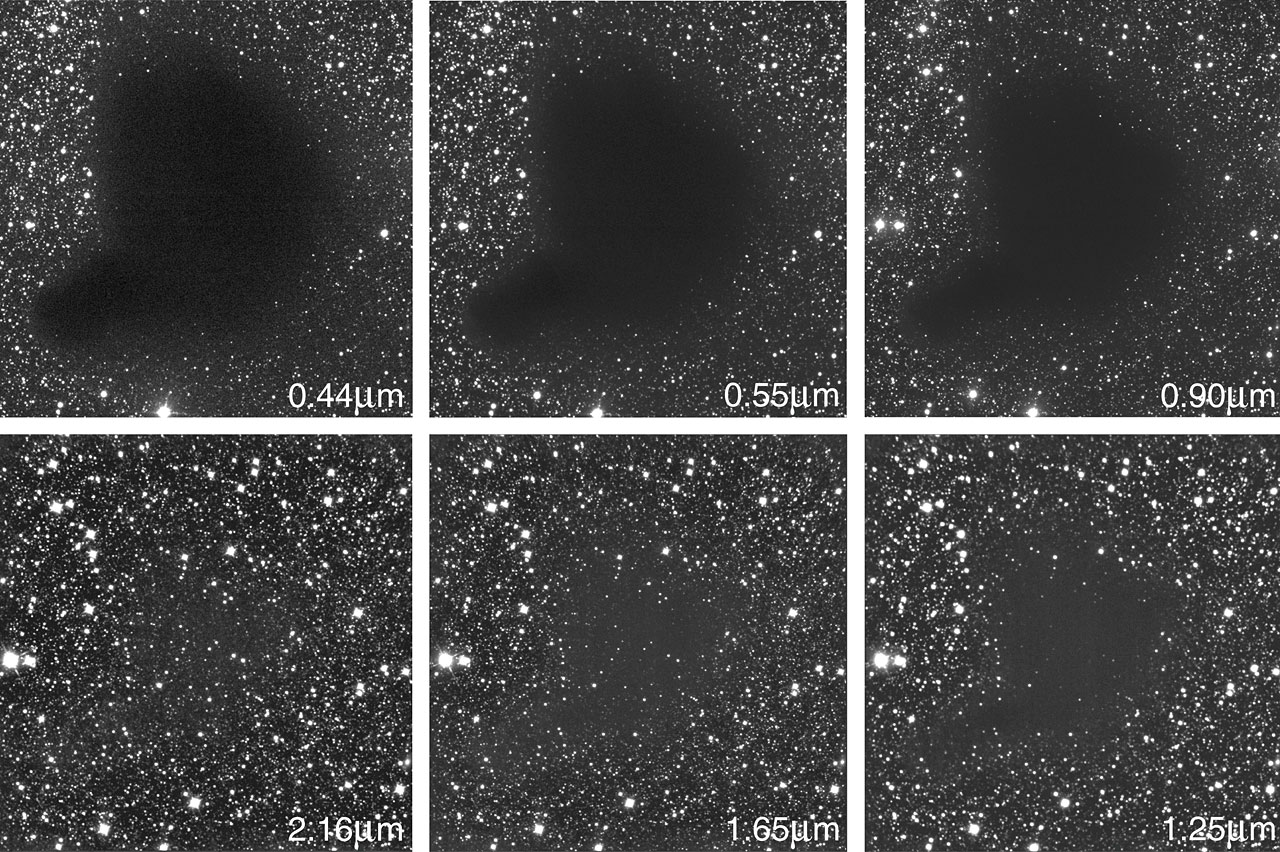
\includegraphics[width=.8\textwidth]{eso9934b}
    \caption{B68 is a dark cloud situated at a distance of about 500~light-years
    (\SI{160}{\parsec})
    towards the southern constellation Ophiuchus.
    This image represents the sky area of the so-called Bok globule Barnard 68 --- nicknamed the Dark Cloud --- imaged in six different wavebands, clockwise from the blue to the near-infrared spectral region.
    Three of these frames
        (``blue'' B-band at wavelength~\SI{0.44}{\micro\meter};
         ``green-yellow'' V-band at~\SI{0.55}{\micro\meter};
         near-infrared I-band at~\SI{0.90}{\micro\meter})
    were obtained with the FORS1 instrument at the VLT ANTU telescope and three with SOFI at the NTT through near-infrared filters
    (J-band at \SI{1.25}{\micro\meter};
    H-band at \SI{1.65}{\micro\meter};
    Ks-band at \SI{2.16}{\micro\meter}).
    It is evident that the obscuration caused by the cloud diminishes dramatically with increasing wavelength.
    Since the outer regions of the cloud are less dense than the inner ones, the apparent size of the cloud also decreases, as more background stars shine through the outer parts.
    Each frame covers an area of
    $4.9 \times 4.9 \operatorname{arcmin^2}$.
    North is up and East is left.  Credit: ESO.}
    \label{fig:dark_cloud}
\end{figure}
\begin{figure}
    \centering
    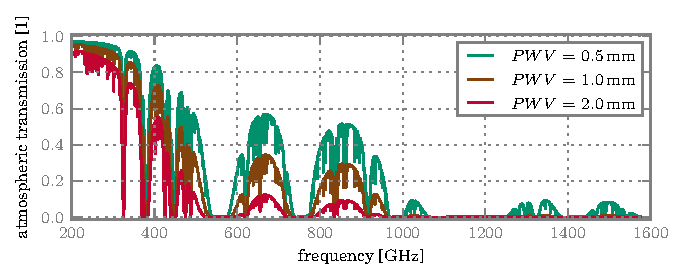
\includegraphics{atmos_trans}
    \caption{
        Atmospheric transmission in the submillimeter domain
        for three Perceptible Water Vapor contents.
        These values are representative of the atmospheric conditions
        at the Chajnantor plateau, home of the
        Atacama Large Millimeter/submillimeter Array (ALMA).
        Its exceptionally arid climate and high altitude (\SI{5000}{\meter}) make
        this location
        one of the best for ground-based submillimeter astronomy.
        Modeled with the \textit{am} transmission model~\parencite{pardo2001atmospheric}.
    }
    \label{fig:atmospheric_electromagnetic_transmission}
\end{figure}

\begin{samepage}
Dense molecular clouds can be best observed in the far-infrared and submillimeter regions of the electromagnetic spectrum:
\begin{itemize}
    \item molecules with a permanent dipole moment (\ce{CO}, \ce{H2O}, etc.) that collide with~\ce{H2} can undergo a transition of their quantized rotational state and emit photons in this domain;
    \item Planck's law peaks in this region for temperatures between~\num{5} and~\SI{100}{\kelvin};
    \item and dust is transparent.
\end{itemize}
\end{samepage}
Unfortunately, the high quantity of water vapor in Earth's atmosphere causes it to absorb most of the submillimetric photons (see~\cref{fig:atmospheric_electromagnetic_transmission}).
Star-forming regions are invisible.

Finally, the technology capable of detecting this radiation was unavailable until the 1990's.

To explain our very existence, astronomers endeavor to solve the problem of star formation,
an unstable cosmic-sized puzzle with ever-moving microscopic evolving pieces.
For too long, they had to solve it in the dark.

%=============================================================================
\subsection{Observatories}

Over the past few decades, the progress in cryogenics and semiconductor technology produced detectors that have the sensitivity required to observe the faint emission from cold molecular clouds: the far-infrared and submillimetric windows were opened.

Placing a telescope in space is ideal to avoid the atmospheric noise and absorption but other factors enter the equation.
Observing the cold universe requires a cold telescope; space observatories were launched with a limited supply of liquid helium which limited their lifetime to about five years (not a limitation anymore thanks to the progress in closed-cycle cooling).
Their spatial resolution is limited by the diameter of their main dish, which is limited by the fairing of the rocket used for the launch (unless the mirror is modular, see JWST~\parencite{lightsey2012james} or Millimetron~\parencite{wild2009millimetron}).
They are expensive: space telescopes must survive a rocket launch, must never break down, and must be mostly autonomous.
Ground-based observation is possible for some wavelengths at high altitude,
what ground telescopes may lack in sensitivity or coverage, they make up in spatial resolution.

Below is a non-exhaustive list of influential submillimeter observatories that have contributed, or are contributing, to our understanding of the complex chemistry of the cold universe.

\begin{samepage}
Ground-based single-dish telescopes:
\begin{itemize}[noitemsep]
    \item 1985: Kölner Observatorium für SubMillimeter Astronomie \parencite{kramer1998new},
    \item 1986: Caltech Submillimeter Observatory   \parencite{murdin2000caltech},
    \item 1987: IRAM 30-meter Telescope             \parencite{baars1987iram}.
\end{itemize}
\end{samepage}

\begin{samepage}
Ground-based interferometers:
\begin{itemize}[noitemsep]
    \item 1992: IRAM Plateau de Bure             \parencite{guilloteau1992iram},
    \item 2004: SubMillimeter Array              \parencite{ho2004submillimeter}, and
    \item 2011: Atacama Large Millimeter Array   \parencite{wootten2009atacama}.
\end{itemize}
\end{samepage}

\begin{samepage}
Airborne observatories:
\begin{itemize}[noitemsep]
    \item 1975: Kuiper Airborne Observatory                      \parencite{gillespie1981kuiper}, and
    \item 2010: Stratospheric Observatory for Infrared Astronomy\\ \parencite{becklin2012stratospheric}.
\end{itemize}
\end{samepage}

\begin{samepage}
Space missions:
\begin{itemize}[noitemsep]
    \item 1995: Infrared Space Observatory  \parencite{isoHandbook1},
    \item 2003: Spitzer Space Telescope     \parencite{werner2004spitzer}, and
    \item 2009: Herschel Space Observatory  \parencite{AA_518_L1}.
\end{itemize}
\end{samepage}



%#############################################################################
\FloatBarrier
\section{The Herschel Space Observatory}

The Herschel Space Observatory~\parencite{AA_518_L1}
shown on~\cref{fig:herschel_spacecraft_artist},
was built and launched with the purpose of studying the cold universe.
It was in operation from 2009 to 2013.


%=============================================================================
\subsection{The satellite}

The Herschel spacecraft was designed, built, tested, and launched under a contract to ESA managed by the Herschel/Planck Project team by an industrial consortium under the overall responsibility of the prime contractor Thales Alenia Space (Cannes), and including Astrium (Friedrichshafen) responsible for the payload module and for system testing at spacecraft level, Thales Alenia Space (Turin) responsible for the service module, and Astrium (Toulouse) responsible for the telescope, with in excess of a hundred subcontractors.

The ``Far Infrared and Sub-millimetre Telescope'' (FIRST) was proposed to the European Space Agency (ESA) in~1982.
After a call for a ``High Throughput Heterodyne Spectroscopy'' in 1984,
ESA considered FIRST in 1986 as one of the four ``cornerstone missions'' of its ``Horizon 2000'' long-term plan~\parencite{pilbratt1997first}.
After a feasibility study, the project was approved in~1993.

In 1999, the design of its payload was approved.
In addition to HIFI, which implements the ``High Throughput Heterodyne Spectroscopy'' that was called for, two spectro-imagers were included.

In 2000 FIRST was renamed ``Herschel Space Observatory'' (HSO), after Friedrich Wilhelm Herschel who discovered the existence of infrared radiation in 1800 (\cref{fig:herschel_discovers_infrared}).

Construction started in 2001 in institutes around the globe.
HIFI was integrated at SRON-Groningen then shipped to ESA's technical center (ESTEC) in 2007 to become part of Herschel.
After passing the tests in the Large Space Simulator of ESTEC, Herschel was flown to Kourou, French Guiana, by an Antonov aircraft.
On the 14\textsuperscript{th} of May 2009, an Ariane~5 rocket lifted Herschel out of Earth's atmosphere.

\begin{figure}
    \centering
    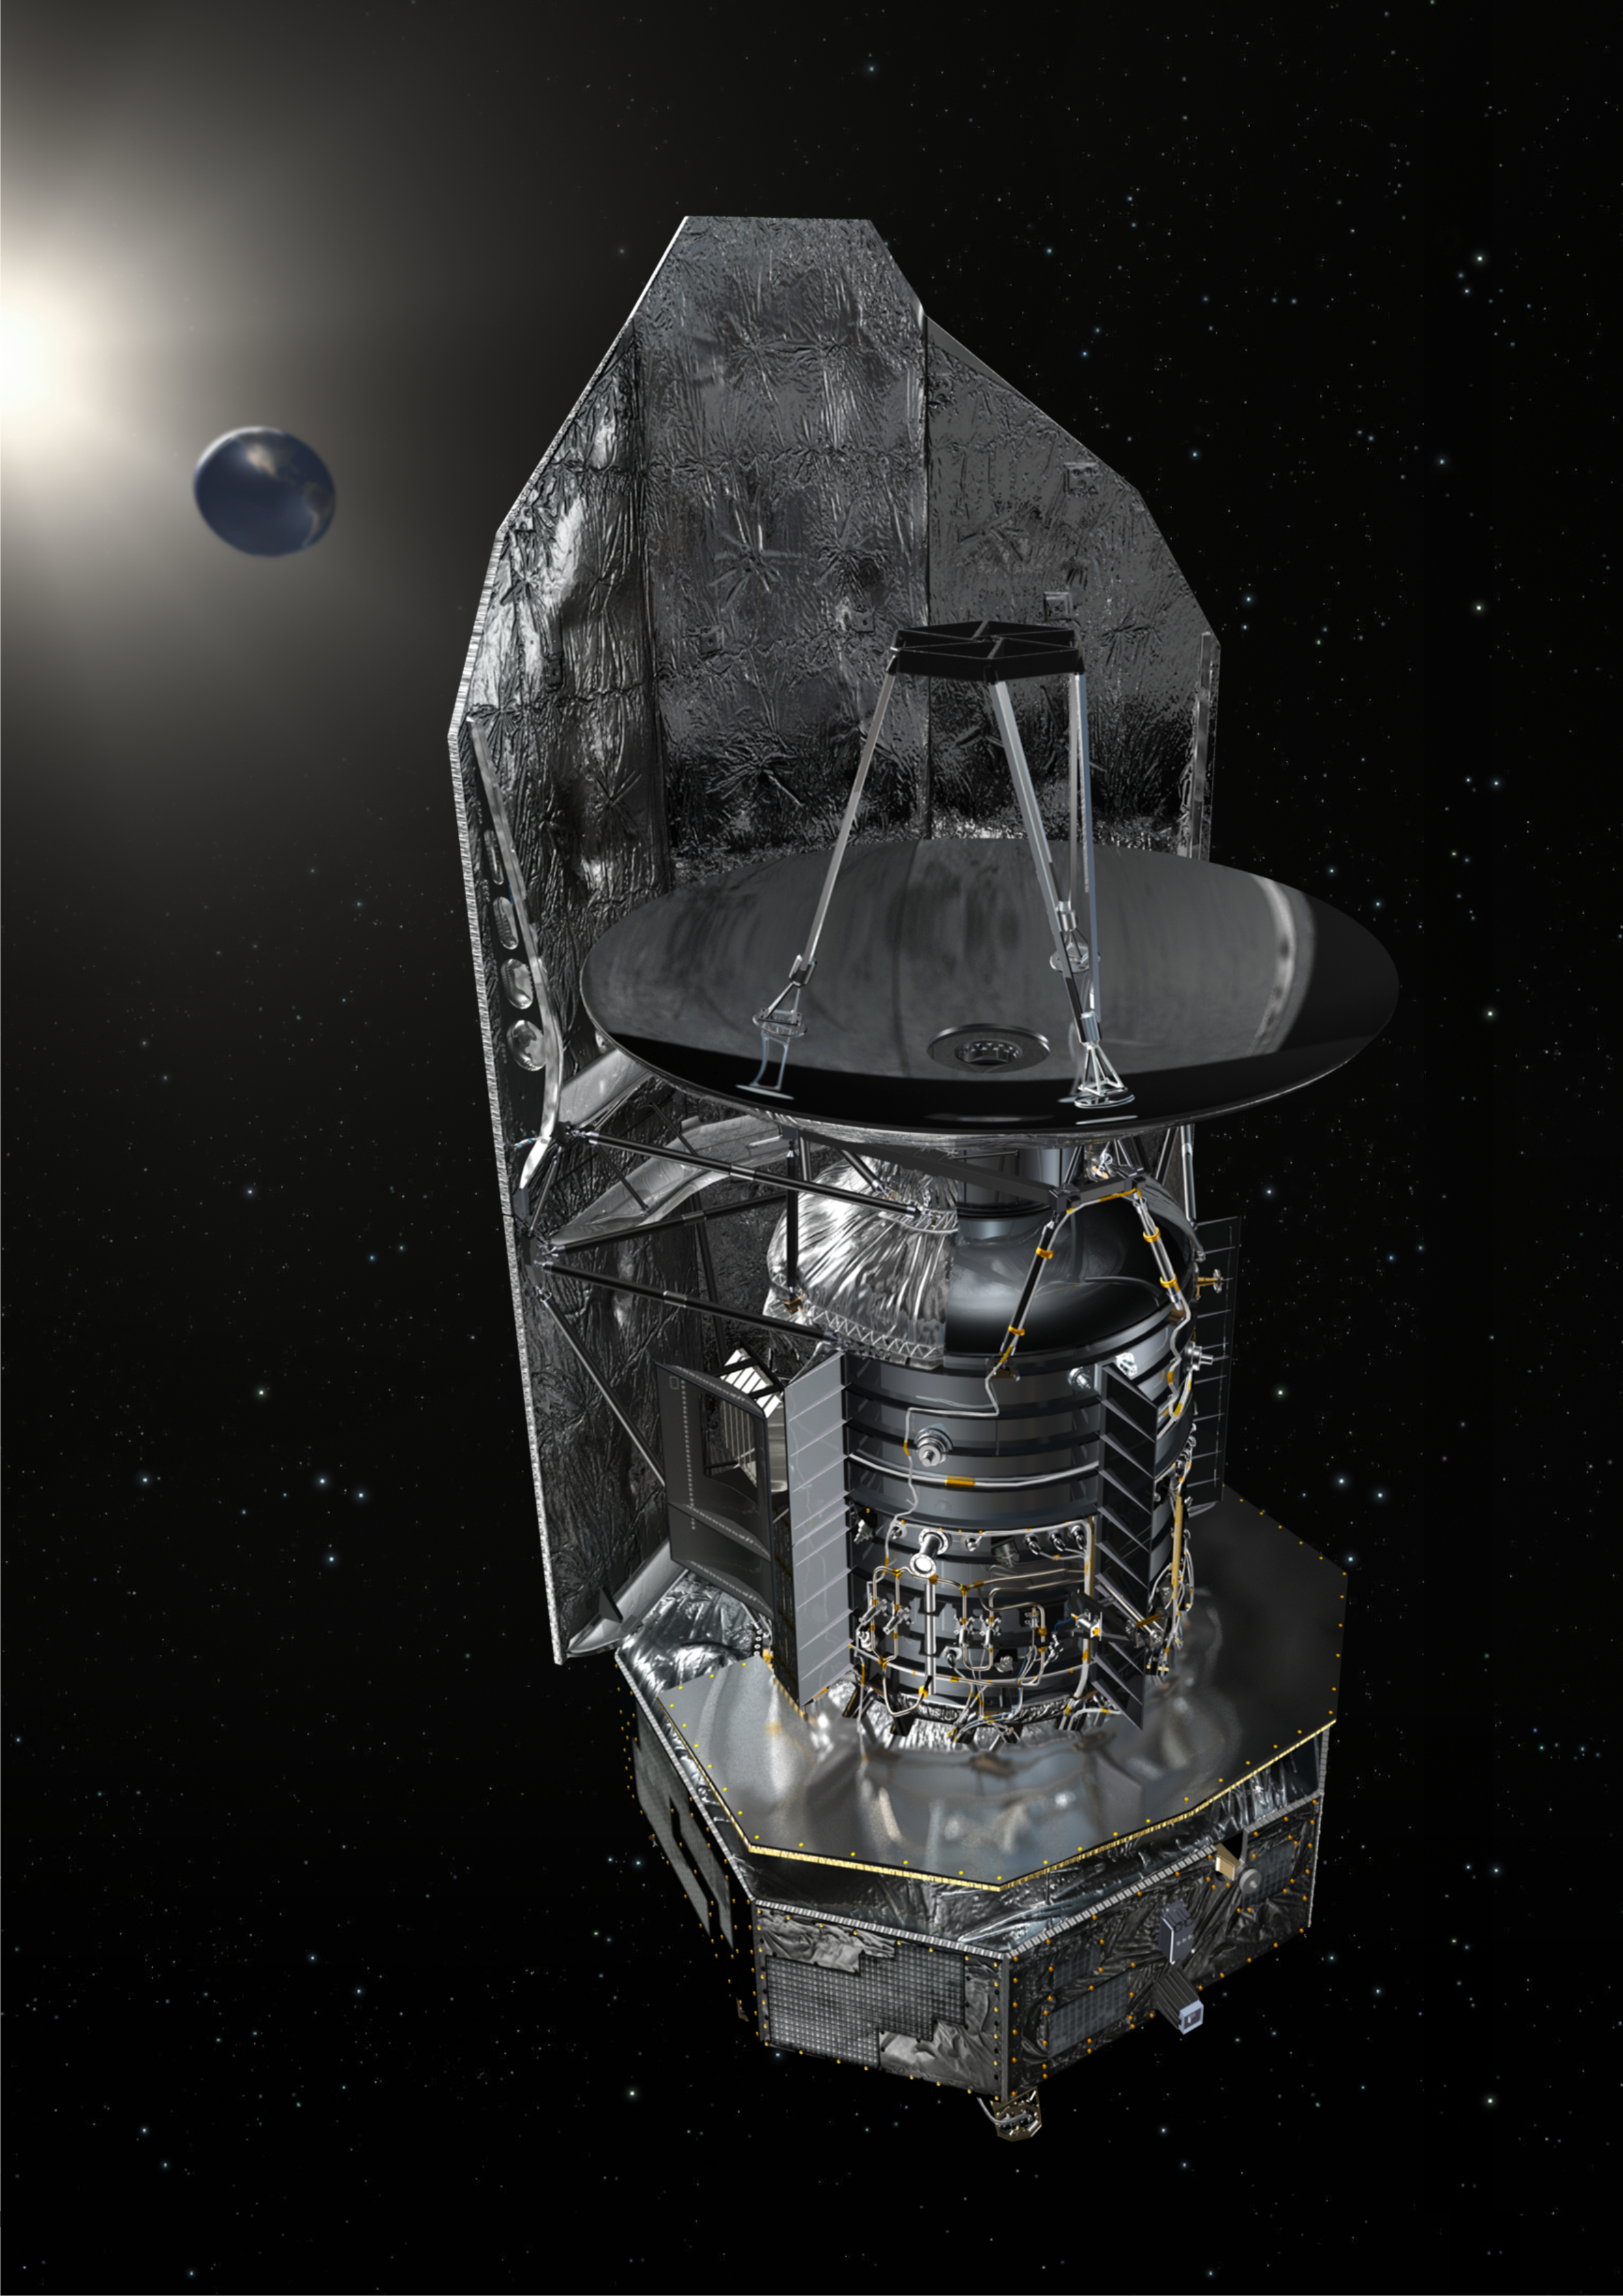
\includegraphics[height=8cm]{herschel_spacecraft_artist}
    \caption{Artist's impression of the Herschel Space Observatory orbiting the Lagrange point $\text{L}_2$ of the Sun--Earth system.
    Image: ESA/AOES Medialab.}
    \label{fig:herschel_spacecraft_artist}
\end{figure}
\begin{figure}
    \centering
    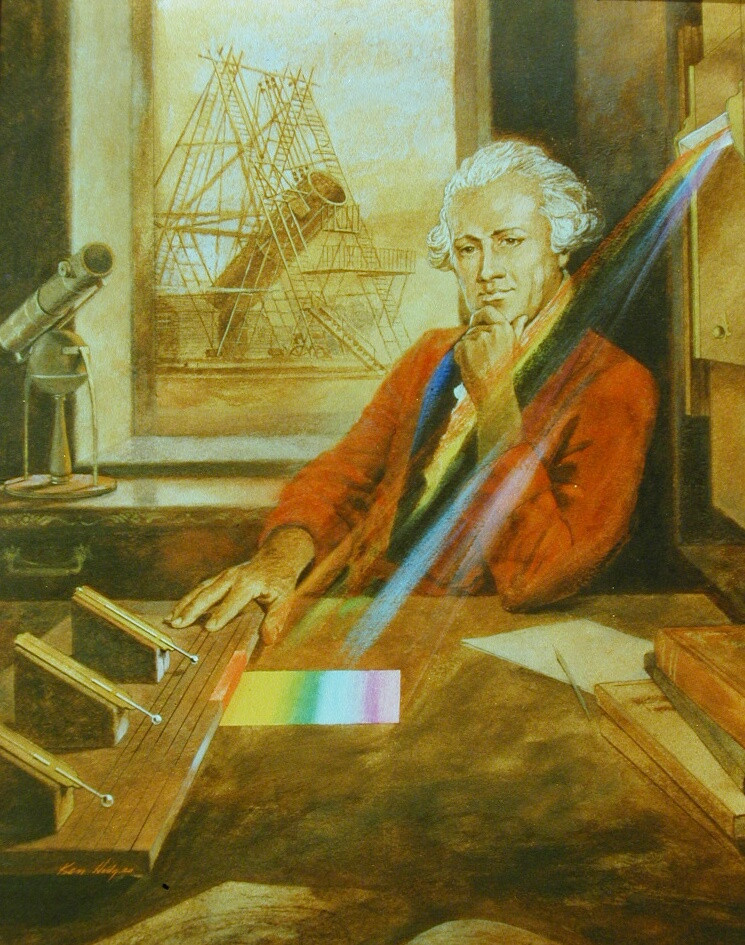
\includegraphics[height=7cm]{herschel_discovers_infrared}
    \caption{Herschel discovering infrared radiation.
        A prism decomposes the sunlight.
        The thermometer does not receive any visible sunlight but registers an elevation of temperature nonetheless:
        the sun emits an invisible radiation beyond the red color.
        Painting: Ken Hodges, 19\textsuperscript{th} century.
    }
    \label{fig:herschel_discovers_infrared}
\end{figure}
\begin{figure}
    \centering
    \includegraphics[width=.5\textwidth]{herschel_s_cryostat_vacuum_vessel}
    \caption{The Herschel cryostat vacuum vessel, seen here in the ESTEC cleanroom, stores 2370 liters of superfluid liquid helium (He II) which is used to help cool the various elements of the detector plane. In orbit, the black outer half of the vessel faces away from the Sun and acts as a radiator while the reflective half faces the inside of the sunshade and reflects excess heat.  Photo: ESA, 2007.}
    \label{fig:photo_hifi_cryo}
\end{figure}
\begin{figure}
    \centering
    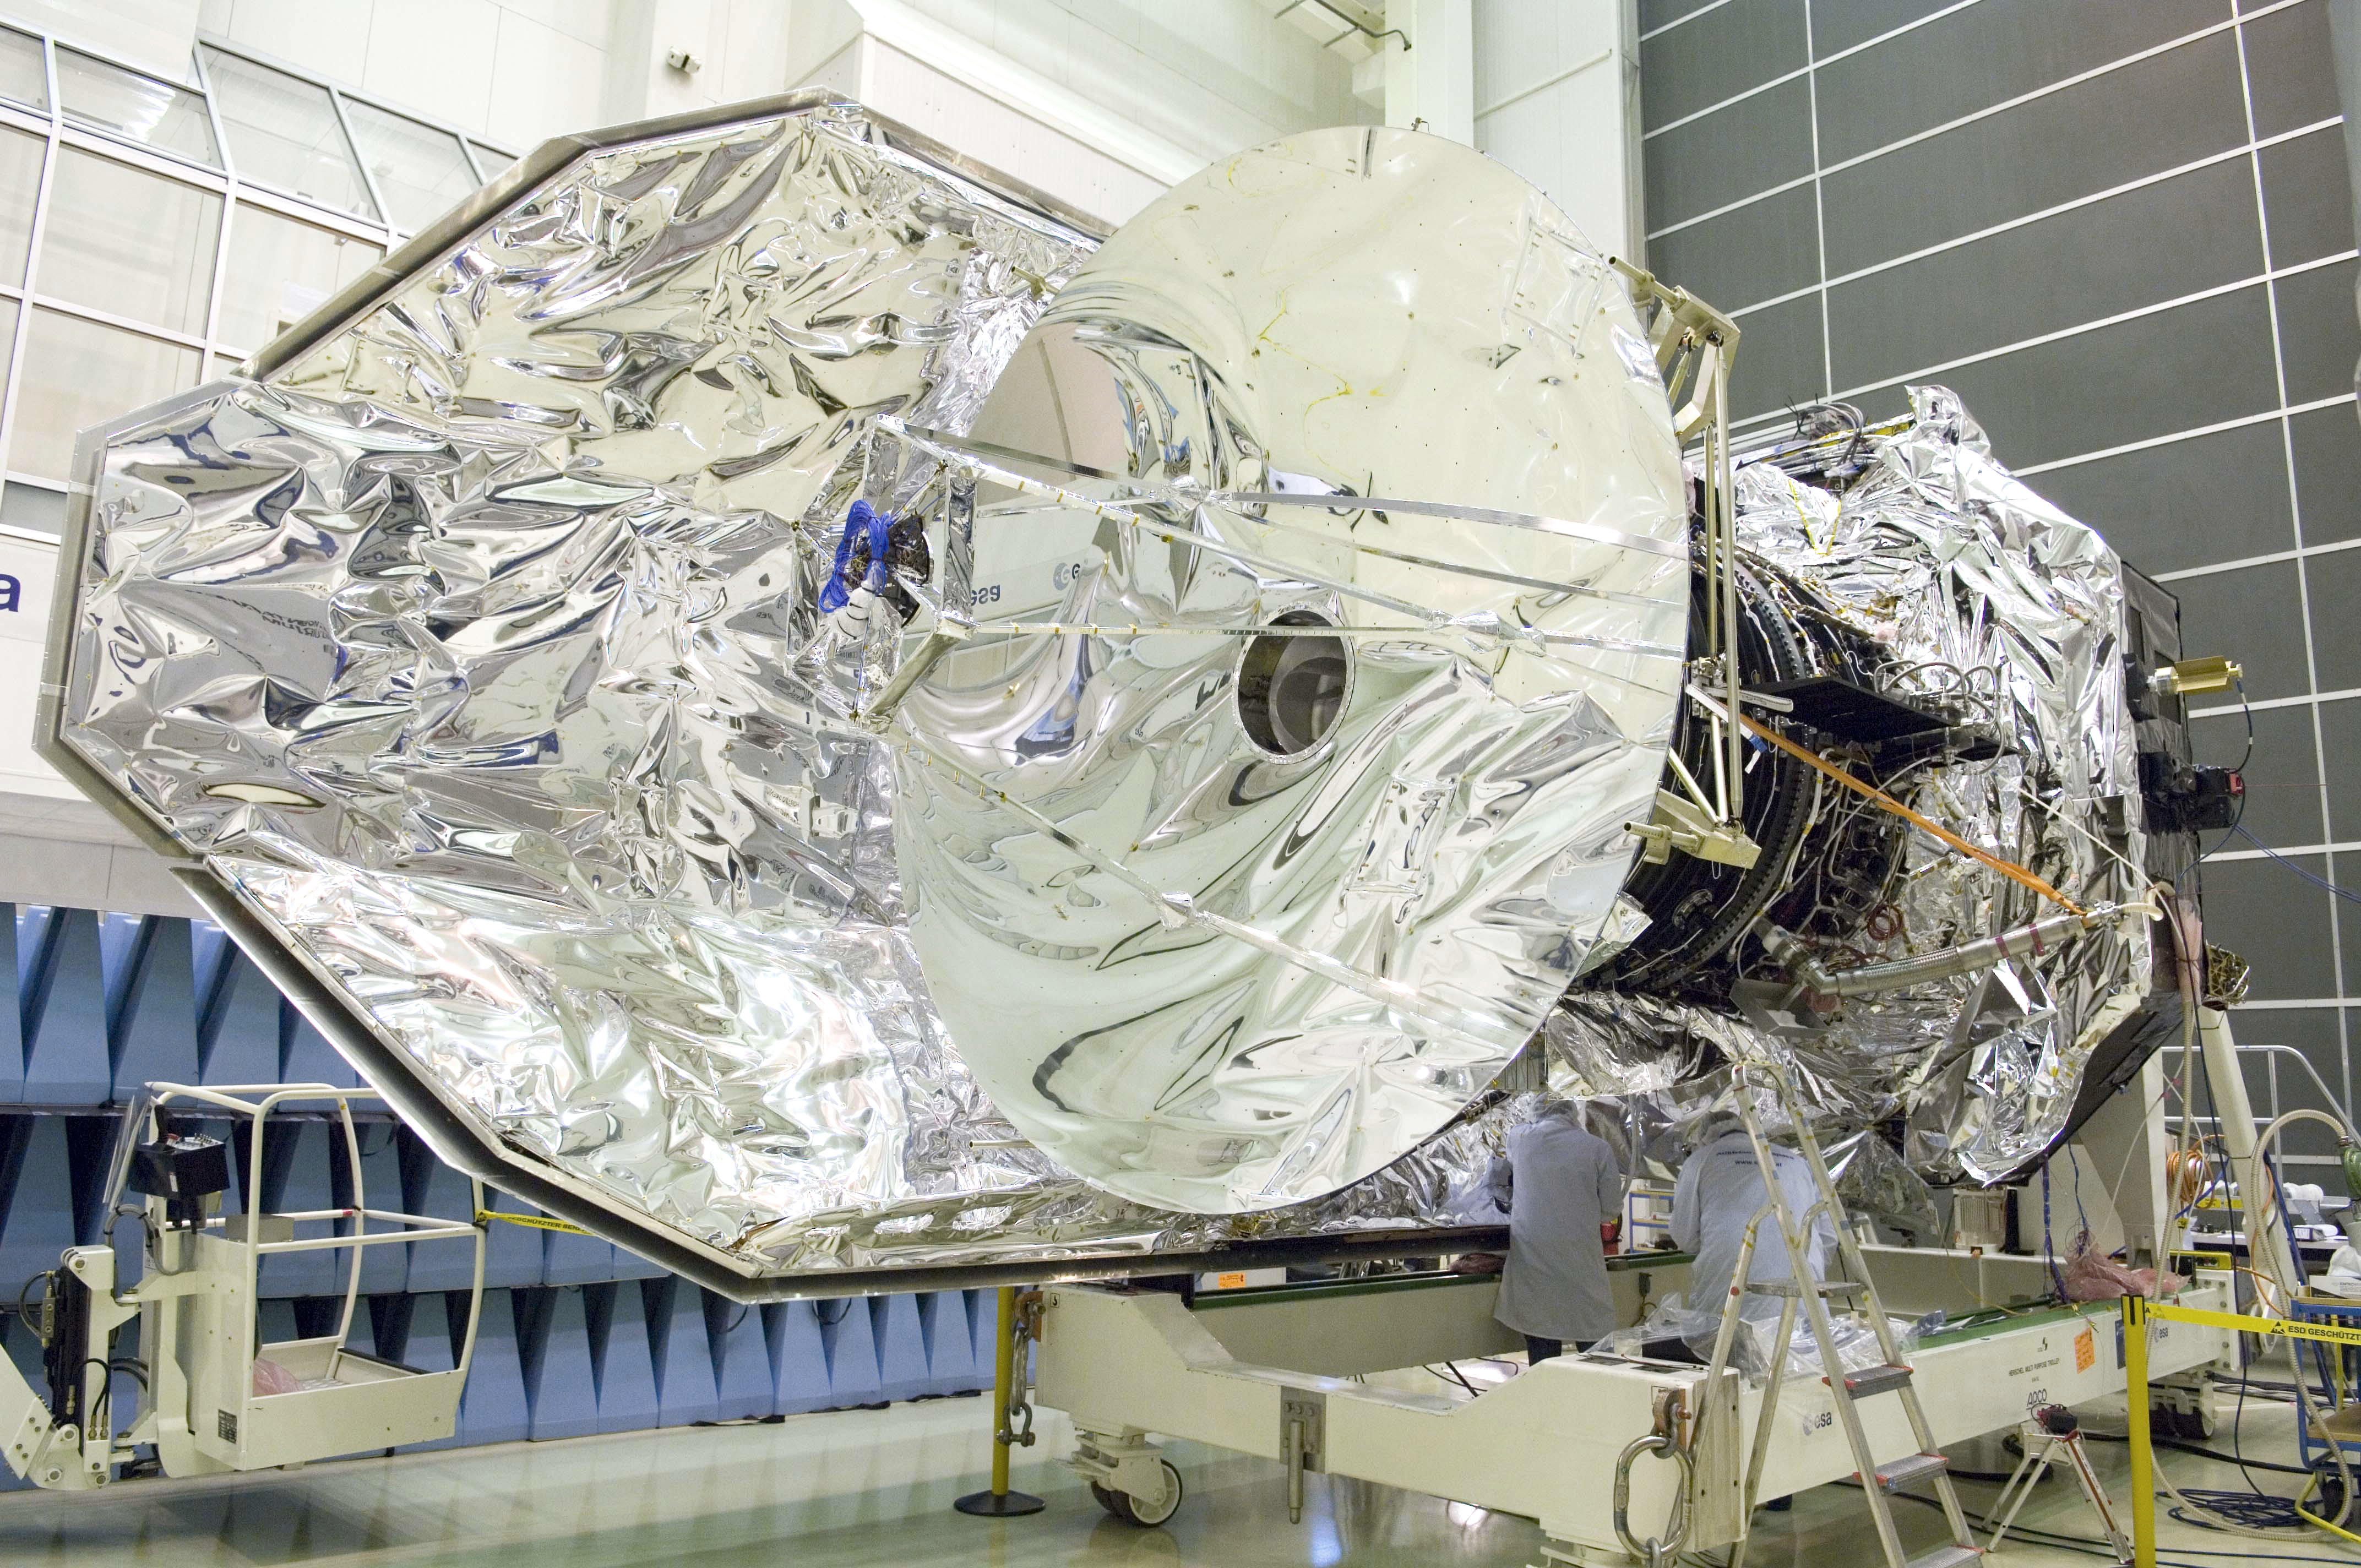
\includegraphics[width=.8\textwidth]{herschel_spacecraft}
    \caption{The flight model of the Herschel spacecraft mounted on its multipurpose trolley in a horizontal position for the the high-precision measurements of the distance between its primary and secondary mirrors (M1 and M2).  Photo: ESA, 2009.}
    \label{fig:photo_herschel}
\end{figure}


During its operation, Herschel was orbiting the Lagrangian point $\text{L}_2$ of the Sun--Earth system, 1.5 million kilometers away from Earth (4~times the distance between Earth and the Moon).
The $\text{L}_2$ point lies on the line going through the two large masses, beyond the smaller of the two (\cref{fig:herschel_spacecraft_artist}).
At $\text{L}_2$, the gravitational forces of the two large masses balance the centrifugal effect.
The Sun--Earth $\text{L}_2$ is a good spot for space-based observatories.
Because an object around $\text{L}_2$ will maintain the same relative position with respect to the Sun and Earth, radiation shielding and calibration are much simpler.
$\text{L}_2$ is too far away from Earth to be affected by its shadow;
this enables Herschel to use solar panels to convert sunlight into energy
but it also warms up the satellite.

Observing the cold universe with a warm telescope is like observing faint stars in broad daylight.
To prevent that, the instruments of Herschel are cooled down in a superfluid helium cryostat\index{cryostat} (\cref{fig:photo_hifi_cryo}).
The cryostat provides temperature between~\SI{1.7}{\kelvin} at its coolest point, up to \SI{10}{\kelvin} where lower temperatures are not required.
The primary mirror itself is not actively cooled down but is shielded from direct sunlight by a sun shade; it has a temperature of approximately~\SI{70}{\kelvin}.

With \SI{2300}{\liter} of Helium on board slowly boiling off at \SI{1.4}{\kelvin}, the mission had a predicted life time of 3.5~years.
Herschel exceeded that requirement by remaining in operation 3.96~years.
Herschel was deorbited from $\text{L}_2$ on the 29\textsuperscript{th} of April 2013 and is now parked on a solar orbit, all its electronics (including communication) shut down.



Herschel's primary mirror\index{mirror, primary} has a diameter of~\SI{3.5}{\meter}, which makes Herschel the largest telescope ever launched in space at the time of writing (2015).
With a mass of~\SI{3300}{\kilo\gram}, it is also the heaviest.
\Cref{fig:photo_herschel} shows a photograph of the HSO at the European Space Research and Technology Center (ESTEC), with engineers for scale.
In comparison, the Hubble Space Telescope has a diameter of~\SI{2.4}{\meter} but operates in the optical band.
In infrared, the other telescopes
are
the Infrared Space Observatory\index{ISO} (ISO)~\parencite{isoHandbook1}
and
Spitzer\index{Spitzer}~\parencite{werner2004spitzer}
with primary mirror diameters of~\SI{60}{\centi\meter} and~\SI{85}{\centi\meter}, respectively.
The diameter of Herschel gives it a sensitivity and a spatial resolution that had never been achieved at these wavelengths.
That diameter was limited only by the size of the fairing of rocket.

%=============================================================================

\subsection{Herschel's scientific instruments}

The Herschel Space Observatory carries three scientific instruments: PACS, SPIRE and HIFI.
PACS and SPIRE are both  spectro-imagers, they complement each other and can be operated simultaneously with a dedicated ``parallel mode'' observing mode.
HIFI stands apart, as a single-pixel high-resolution spectrometer.

%-----------------------------------------------------------------------------
\subsubsection{PACS}
\index{PACS}The Photodetecting Array Camera and Spectrometer%
~\parencite{poglitsch2010photodetector}
comprises two mutually exclusive sub-instruments: a bolometric camera to perform photometry in three spectral bands (\num{70}, \num{100} and \SI{160}{\micro\meter}) and an integral field unit grating spectrometer operating over the spectral range from~\num{57} to~\SI{210}{\micro\meter} with a spectral resolution ranging from~\num{1000} to~\num{5000}.

The camera of PACS (see~\cref{fig:m51_pacs_composite}) revealed the ubiquity of the filamentary structure of star forming regions~\parencite{2010A&A...518L.100M}.

The spectrometer of PACS provides information on the abundances of molecules
(\ce{CO}, \ce{H2O}, \ce{OH}) atomic species (\ce{O+}, \ce{O^2+}, \ce{C+}) and continuum.
This can be used for instance to determine which of these spectral lines are efficient at cooling the gas in star forming regions~\parencite{2013A&A...552A.141K}.

\begin{figure}
    \centering
    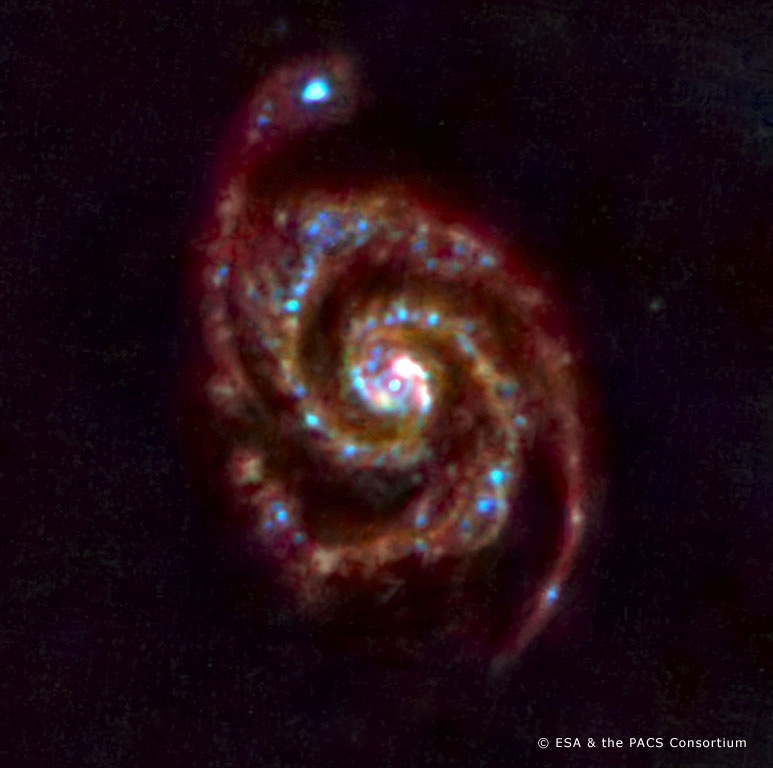
\includegraphics[width=.6\textwidth]{m51_pacs_composite}
    \caption{
        Three-color far-infrared image of M51, the ``whirlpool galaxy''.
        Red, green and blue correspond to the \SI{160}{\micro\meter}, \SI{100}{\micro\meter} and \SI{70}{\micro\meter} wavelength bands
        of Herschel-PACS.
        Blue indicates regions of warm dust that is heated by young stars, while the colder dust shows up in red.
        This image was taken on Herschel's first operational day (14 June 2009).
        Credit: ESA and the PACS Consortium.
    }
    \label{fig:m51_pacs_composite}
\end{figure}

%-----------------------------------------------------------------------------
\subsubsection{SPIRE}
\index{SPIRE}The Spectral and Photometric Imaging Receiver%
~\cite{griffin2010herschel}
is also an imaging camera and a low-resolution spectrometer.
The bolometric camera has three bands centered at \num{250}, \num{350} and~\SI{500}{\micro\meter}.
The spectrometer has a resolution between \num{40} and~\num{1000} at~\SI{250}{\micro\meter}.

SPIRE operates at longer wavelengths than PACS, which explains in part its lower spatial resolution and wider field of view.
This also gives SPIRE a higher sensitivity and makes this instrument suitable for observing faint extragalactic sources.

The Herschel Multi-tiered Extragalactic Survey (HerMES) focused on SPIRE data to investigate the formation of galaxies at high redshift~\parencite{oliver2012herschel}.
SPIRE also contributed to the study of Active Galactic Nuclei~\parencite{hatziminaoglou2010hermes}, quasars~\parencite{bonfield2011herschel} and massive black holes~\parencite{van2010black}.

%-----------------------------------------------------------------------------
\subsubsection{HIFI}
\index{HIFI}The Heterodyne Instrument for the Far Infrared%
~\parencite{AA_537_A17}
is a single-pixel high-resolution spectrometer.
It operates between~\num{157} and~\SI{650}{\micro\meter} and its spectral resolution can reach~\num{1.5e6}.

A summary of the first three years of HIFI results can be found in~\textcite{vandertak2012first}.
Among them,
the discovery of interstellar chloronium~\parencite{lis2010herschel},
of a new population of ``warm dark'' interstellar molecular clouds devoid of~\ce{CO}~\parencite{langer2010c+},
of planets currently forming in the accretion disk of DM Tau~\parencite{bergin2010sensitive}, etc.
Later, HIFI discovered water on Ceres~\parencite{kuppers2014localized},
solved a chronological question related to the youth of our solar system~\parencite{ceccarelli2014herschel},
demonstrated (with PACS) that the high-altitude water content in Jupiter originated from the impact of Shoemaker-Levy~9 in 1994~\parencite{cavalie2013spatial}, etc.

The next section focuses on HIFI, its technology and its calibration.


%#############################################################################

\section{HIFI}

The Heterodyne Instrument for the Far Infrared (HIFI) operates at frequencies between \SI{480}{\giga\hertz} and \SI{1910}{\giga\hertz},
producing spectra with a resolution ranging from \SI{1}{\mega\hertz} to \SI{125}{\kilo\hertz}~\parencite{AA_518_L6}.

This high frequency resolution enables astronomers to study, not only the abundance of chemical species, but also the kinematic properties of their environment.

The Low Energy Astrophysics (LEA) division of the Netherlands Institute for Space Research (SRON%
\footnote{
    Stichting Ruimte Onderzoek Nederland.
    \url{https://www.sron.nl/}
}%
) located in Groningen (The Netherlands)
had accumulated a valuable expertise in space infrared spectroscopy by developing
LRS for IRAS%
\footnote{
    IRAS LRS: Infrared Astronomical Satellite, Low Resolution Spectrometer~\parencite{neugebauer1984infrared}
}
and SWS for ISO%
\footnote{
   ISO SWS: Infrared Space Observatory, Short Wavelength Spectrometer~\parencite{isoHandbook5}.
}%
;
it became the Principal Investigator Institute under the leadership of Thijs de Graauw, and later Frank Helmich.

HIFI has been designed and built by a consortium of institutes and university departments from across Europe, Canada and the USA, with major contributions from Germany, France and the USA. Consortium members are: Canada: CSA, U.Waterloo; France: CESR, LAB, LERMA, IRAM; Germany: KOSMA, MPIfR, MPS; Ireland, NUI Maynooth; Italy: ASI, IFSI-INAF, Osservatorio Astrofisico di Arcetri-INAF; Netherlands: SRON, TUD; Poland: CAMK, CBK; Spain: OAN(IGN), CAB(CSIC-INTA); Sweden: Chalmers University of Technology - MC2, RSS \& GARD; OSO; SNSB, Stockholm University - SO; Switzerland: ETH Zurich, FHNW; USA: Caltech, JPL, NHSC.

%\Cref{fig:prismas,fig:hexos} illustrate the sensitivity, coverage and resolution of HIFI.
%\begin{figure}
%    \centering
%    \includegraphics[scale=0.8]{prismas}
%    \caption{Selection of HIFI spectra towards (a) W49N and (b) W51, two star-forming regions. The spectra have been normalized to the continuum to emphasize the absorption profiles, and shifted vertically to avoid overlap.
%    The~\ce{C+} fine-structure line occurs at~\SI{1.9}{\tera\hertz}.
%    Credit:~\parencite{gerin2012hydride}.
%    }
%    \label{fig:prismas}
%\end{figure}
%\begin{figure}
%    \centering
%    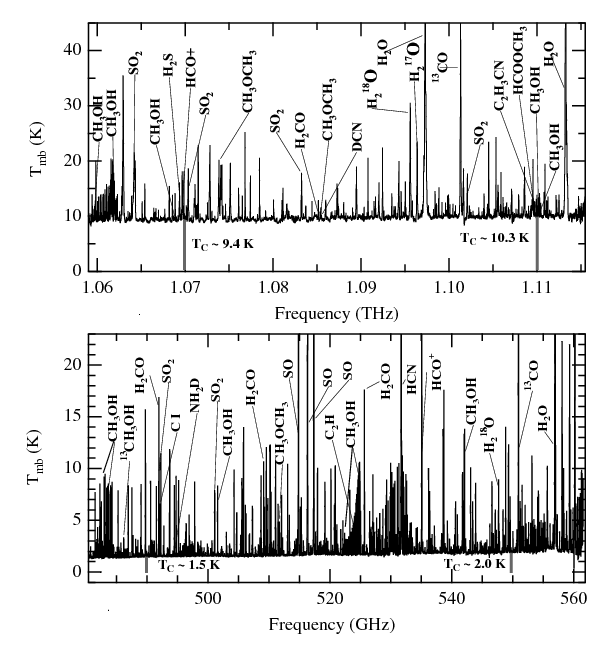
\includegraphics[width=.8\textwidth]{hifi_hexos}
%    \caption{Top: HIFI spectral scan of Orion KL in Band 4b. Bottom: HIFI spectral scan of Orion KL in Band 1a. Strong lines in both spectra are identified.  Credit:~\parencite{bergin2010herschel}.
%    }
%    \label{fig:hexos}
%\end{figure}

%=============================================================================

\subsection{The problem of ripples}

Despite the careful design of HIFI,
its spectra can show ripples, examples of which are shown in~\cref{fig:ripples}.
The baseline of these spectra should be flat but instead shows oscillations that have a period of about~\SI{100}{\mega\hertz}.
The absence of visible ripples on the continuum does not guarantee that the intensity and/or the profile of the lines is correct.
These ripples constitute a major source of uncertainty, as we show in~\cref{sec:intensity_calibration}.

This is an instrumental artifact resulting from electromagnetic interferences inside cavities formed by various optical element of HIFI.

In this thesis, I present the physically-based technique that I developed to model interferences and predict the gain of a coherent optical system.

\begin{figure}[bp]
    \centering
    \includegraphics[width=.8\textwidth]{mars_50010cb7_WBSH_USB}
    \caption*{Continuum and absorption line of Mars.
              Source: HSA obsid~0x50010cb7.
    }
    \bigskip
    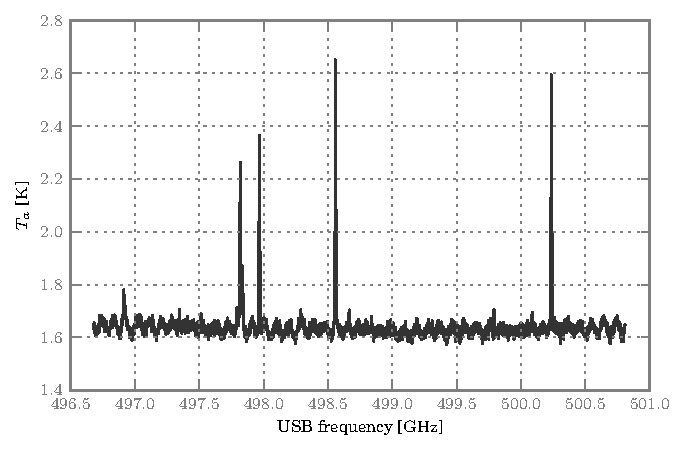
\includegraphics[width=.8\textwidth]{50003791_00}
    \caption*{Continuum and emission lines in Orion S.
       Source: HSA obsid~0x50003791, credit:~\textcite{goldsmith2011herschel}.}
    \caption{Two examples of ripples caused by interferences in the optics of HIFI.}
    \label{fig:ripples}
\end{figure}



%=============================================================================
%\FloatBarrier
\subsection{Heterodyne detection}

%-----------------------------------------------------------------------------

\subsubsection{Principle}
The technology that would allow to build a far-infrared detector with a spectral resolution of~\num{e6} does not exist yet.
However, detectors with a spectral resolution of \num{5e4} or lower can be built at frequencies of a few gigahertz (microwave region of the electromagnetic spectrum).
This is how HIFI achieves its high spectral resolution: it converts the high-frequency signal from the sky down to a lower frequency, for which high-resolution detectors can be built.
The technique used to lower the frequency of the sky signal is called ``heterodyning''.

A heterodyne receiver creates new frequencies by mixing two frequencies.
The mixing is done by a non-linear device called a ``mixer''\index{mixer}.
Typically, a mixer receives two frequencies $f_1$ and $f_2$ and produces two other frequencies $\abs{f_1-f_2}$ and $f_1+f_2$.
One of the two output frequencies is generally discarded, while the other is directed toward a detector.
If $f_1$ is the signal we wish to detect, then we can adjust $f_2$ to bring the $f_1$ down to the frequency range of the detector.
The frequency that the detector receives is fixed, and called the ``Intermediate Frequency'' (IF).

In HIFI, $f_1=f_\text{sky}$ the sky frequency,
and $f_2=f_\text{LO}$ the Local Oscillator frequency.
The mixer output at $f_\text{LO}+f_\text{sky}$ is discarded, such that
the sky, LO and intermediate frequencies are related by
\begin{equation}
    f_\text{IF} = \abs{f_\text{sky} - f_\text{LO}}\text{.} \label{eq:heterodyne_question}
\end{equation}
Each channel of a HIFI spectrum has its own $f_\text{IF}$.
Because of the absolute value, each $f_\text{IF}$ has two matching $f_\text{sky}$:
\begin{equation}
    \begin{aligned}
        f_\text{sky, LSB} &= f_\text{LO} - f_\text{IF}    \text{, and}    \\
        f_\text{sky, USB} &= f_\text{LO} + f_\text{IF}    \text{.}
    \end{aligned}
    \label{eq:sideband_convolution}
\end{equation}
These two frequencies are called the ``lower'' and ``upper sideband frequencies'', both are simultaneously down-converted and contribute to the power detected at $f_\text{IF}$.
A HIFI spectrum is, in fact, a superposition of two spectra, as illustrated by~\cref{fig:heterodyne_principle}.
\begin{figure}
    \centering
    \input{heterodyne_principle.pdf_tex}
    \caption{The heterodyne principle.
        The output of the mixer is a superposition of the lower and upper sidebands of the input, shifted down in frequency.
        Note that the contribution of the LSB is flipped.}
    \label{fig:heterodyne_principle}
\end{figure}

For some applications, it is desirable and possible to filter the sky signal before it hits the mixer in order to reject one sideband.
Such filters did not exist when HIFI was designed and still do not exist in~2015.
Alternatively, one can build the sideband rejection/separation into the mixer itself; ALMA benefits from the most recent advances in sideband-separating mixers.
In HIFI, there is no sideband rejection or separation.
Since HIFI detects both sidebands, it is called a double-sideband receiver.


%-----------------------------------------------------------------------------

\subsubsection{Sideband convolution}

As shown by~\cref{eq:sideband_convolution,fig:heterodyne_principle}, given a single spectrum and no a-priori knowledge about the sky, it is impossible to tell whether a feature seen on a spectrum comes from the LSB, from the USB, or form both and in which proportion.
This degeneracy is called ``sideband convolution''.
Whether sideband convolution is a good thing or not depends on the situation.
\begin{itemize}[noitemsep,nolistsep]
    \item For spectra that have a few narrow predicted lines, convolution is a good thing.
    Quantum mechanics tells us where the lines will appear, it is easy to find a LO frequency that will not introduce any confusion.
    As a result, the frequency coverage is doubled.
    A second advantage is that the continuum is essentially observed twice, which reduces its uncertainty by~$1/\sqrt{2}$.
    \item For line-rich spectra however, such as those generated by complex organic molecules, sideband convolution can become quite confusing.
\end{itemize}

Spectra can be deconvolved by repeating the observation with a different LO frequency.
When the LO frequency increases, lines from the USB move to the left (lower IF) and lines from the LSB to the right (higher IF).
If doing it by eye is too tedious, a sideband deconvolution algorithm can apply this technique to a series of spectra~\parencite{comito2002deconvolution}.
The spectrum presented in~\cref{fig:hexos} was deconvolved with this technique, implemented as a standard step in the automated data-reduction pipeline of HIFI for spectral scans.

\begin{figure}[hbp]
    \centering
    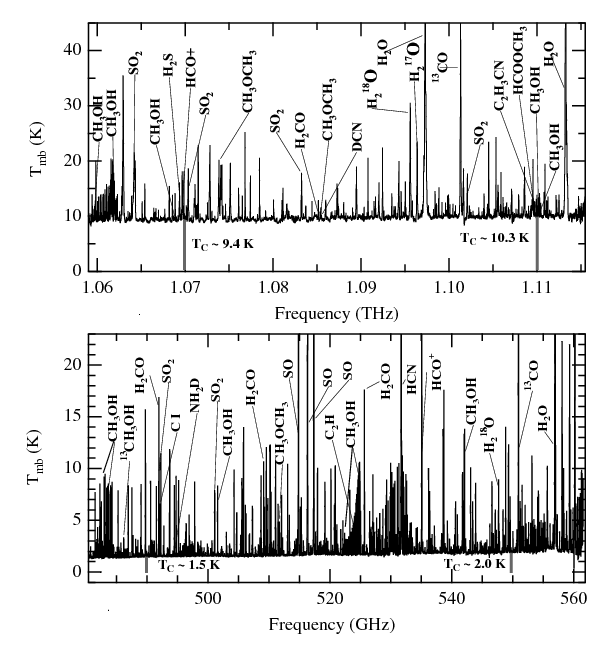
\includegraphics[width=.6\textwidth]{hifi_hexos}
    \caption{Top: HIFI spectral scan of Orion KL in Band~4b. Bottom: HIFI spectral scan of Orion KL in Band 1a. Strong lines in both spectra are identified.  Credit:~\parencite{bergin2010herschel}.
    }
    \label{fig:hexos}
\end{figure}



%-----------------------------------------------------------------------------
\clearpage
\subsubsection{Hardware implementation}

This section gives a very short high-level description of the mixers and local oscillators used in HIFI.
Specifics can be found for example in~\textcites{pearson2000local}{pearson2003terahertz}{jackson2006low} or \textcite{kooi2008}.

\begin{samepage}
HIFI uses two types of mixers:
\begin{itemize}[noitemsep,nolistsep]
    \item Bands~1 to 5 use
Superconductor-Insulator-Superconductor (SIS) junctions that rely on the quantum-tunneling of Cooper pairs of electrons and quasiparticles through the insulator.
    \item Bands~6 and 7 use  Hot Electron Bolometers (HEB) that rely the strongly non-linear temperature-dependence of the resistance of a superconductor as a base for the heterodyne mixing process.
\end{itemize}
\end{samepage}

All the mixers of HIFI are cooled to~\SI{1.7}{\kelvin}, the lowest temperature that the Herschel cryostat can provide.
This keeps them in their superconductor state and reduces the thermal noise, which increases their sensitivity.

HIFI contains 14 mixers: 7 bands and 2 polarizations per band.
The polarization is noted ``H'' for horizontal and ``V'' for vertical.
Each mixer is therefore identified by its band and polarization: 1H, 1V, 2H, 2V, etc.
Only one mixer band is active at a given time but its two mixers are simultaneously active.
These seven bands provide a continuous frequency coverage from \num{480} to \SI{1250}{\giga\hertz} (Bands 1--5) and from \num{1410} to \SI{1910}{\giga\hertz} (Bands 6--7).
\Cref{tab:sevenbands} summarizes the frequencies and technologies used in each band.
The \SI{160}{\giga\hertz}-gap between Band~5 and Band~6 results from technological difficulties: neither SIS nor HEB had satisfying performances in this range.

The Local Oscillator Unit (LOU) pumps the mixers to their operation point and provides a phase-locked monochromatic signal for the mixing process.
The HIFI LOU contains 7 cartridges, one per mixer band (see~\cref{fig:photo_hifi_lou}).
Each cartridge contains two signal chains called ``a'' and ``b'', each able to produce power in half of the band.
LO bands are therefore named 1a, 1b, 2a, 2b, etc.
Only one LO band is active at a time.
The LO signal is split by a wire-grid polarizer to illuminate equally the horizontal and vertical mixer.
For example the LO subband 3a is used to pump the mixers 3H and 3V simultaneously anywhere between~\num{800} and \SI{880}{\giga\hertz}.

\begin{table}
    \centering
    \begin{tabular}{ccccc}
        \toprule
        band & freq. range [\si{\giga\hertz}] & LO injection & mixer & coupling \\
        \midrule
        1 &  480--640  & beam splitter & SIS & horn\\
        2 &  640--800  & beam splitter & SIS & horn\\
        3 &  800--960  & diplexer      & SIS & horn\\
        4 &  960--1120 & diplexer      & SIS & horn\\
        5 & 1120--1250 & beam splitter & SIS & lens\\
        6 & 1410--1703 & diplexer      & HEB & lens\\
        7 & 1703--1910 & diplexer      & HEB & lens\\
        \bottomrule
    \end{tabular}
    \caption{Frequency and technology of the seven HIFI bands.}
    \label{tab:sevenbands}
\end{table}
\begin{figure}
    \centering
    \begin{subfigure}[c]{.7\textwidth}
        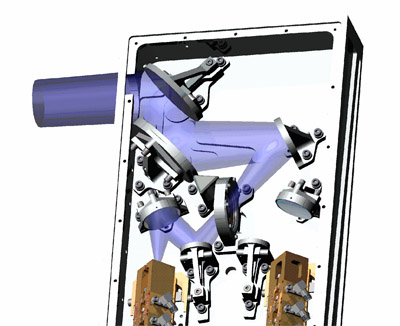
\includegraphics[width=\textwidth]{lou_band_5_drawing}
    \end{subfigure}%
    \begin{subfigure}[c]{.22\textwidth}
        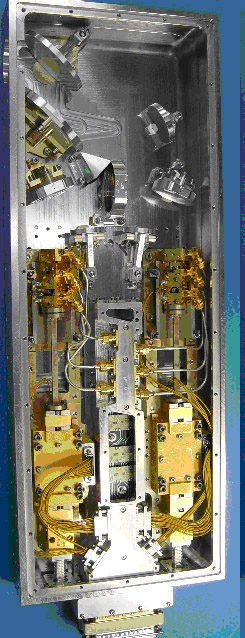
\includegraphics[width=\textwidth]{lou_band_5}%
    \end{subfigure}%
    \caption{
        Drawing and photograph of the HIFI LO flight model cartridge for Band~5.
        Each LO cartridge contains two signal chains (golden),
        bias filtering modules and an optical system.
        Credit: MPIfR.
    }
    \label{fig:photo_hifi_lou}
\end{figure}


%=============================================================================
\subsection{Optics}

\Cref{fig:photo_hifi_fpu} shows the focal plane unit (FPU) of HIFI.
The sky signals enters the instrument on the right side.
On the left side, in red, are the seven windows that are facing the seven local oscillator cartridges.
The FPU is inside the cryostat but the local oscillators are not.
The seven windows in the cryostat are visible on~\cref{fig:photo_hifi_cryo}: 9 holes for 7 local oscillator beams and 2 alignment devices, lined-up horizontally toward the top of the tank.
\Cref{fig:photo_hifi_fpu} also shows the 14 mixer units: 7 on the left above the LO feeds for one polarization, and 7 on top for the other polarization.

\begin{samepage}
Between other things, the focal plane unit is responsible for
\begin{itemize}[nolistsep,noitemsep]
    \item Selecting the source.  An actuated mirror called ``chopper'' rotates to couple the two mixers either to the sky (several sky positions are available) or to internal calibration loads (see \cref{sec:intensity_calibration}).
    \item Splitting each input (source and LO) into two beams, one for each mixer.
    \item Line-up the polarization of the source and LO beams with that of each mixer.
\end{itemize}
\end{samepage}

\begin{figure}
    \centering
    \begin{subfigure}[c]{.4\textwidth}
        \includegraphics[width=\textwidth]{hifi_fpu}
    \end{subfigure}%
    \begin{subfigure}[c]{.6\textwidth}
        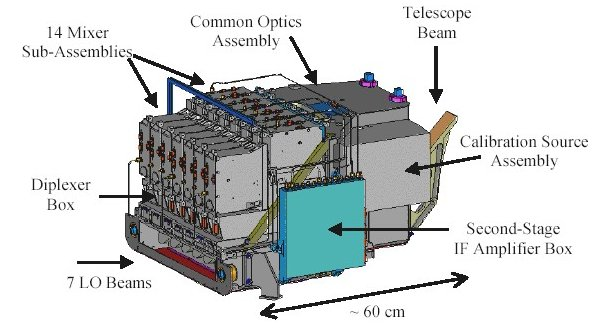
\includegraphics[width=\textwidth]{hifi_fpu_schematic}
    \end{subfigure}
    \caption{HIFI Focal Plane Unit.  Photo: ESA 2007.}
    \label{fig:photo_hifi_fpu}
\end{figure}

HIFI uses two systems for injecting the LO beam inside the sky beam: beam splitters or diplexers.

%-----------------------------------------------------------------------------
\subsubsection{Beam-splitter LO injection}
Band~1, 2 and 5 use an optical configuration based on beam-splitters illustrated in~\cref{fig:beamsplitter_layout}.
In beam splitter bands, the sky and LO beams are split in two by beam splitters.
These beam splitters are not homogeneous dielectric thin films but wire-grid polarizers, which are suitable since the mixers are sensitive to one polarization only.
The inclination of the wires of~Grid~0 is chosen in order to maximize the mixer--sky coupling while minimizing the mixer--LO coupling.
Most of the LO power is transmitted through Grids~H and~V and discarded into absorbers (dumped);
only the minimal amount of power required to pump the mixers to their nominal level is reflected.
In Band~1 for instance, \SI{99}{\percent} of the LO power is dumped.

What might seem at first like a waste of power is in fact a wise and sensible design decision for two reasons.
First, the LO is warm (outside the cryostat, temperature about~\SI{120}{\kelvin}) which makes it a source of thermal noise and therefore background radiation.
The lower the mixer--LO coupling, the lower the background noise.
Second, the lower the coupling, the less interferences: the LO--mixer interferences are so weak that they have no measurable effect on Band~1 spectra.

This optical configuration can couple at most~\SI{50}{\percent} of the LO power;
when the LO power is not abundant enough, another configuration is required.

\begin{figure}
    \centering
    \footnotesize
    \input{band1_layout.pdf_tex}
    \caption{Optical layout of the beam-splitter configuration in Band~1.
    The vertical polarization is in the plane of the page, the horizontal polarization is normal to the plane of the page.
    Dotted lines represent grids, thick full lines represent mirrors, mixers horns are represented by thick V-shaped symbols.
    }
    \label{fig:beamsplitter_layout}
\end{figure}

%-----------------------------------------------------------------------------
\subsubsection{Diplexer LO injection}
\label{sec:diplexer_lo_injection}
The LO power available in Band~3, 4, 6 and 7 is so low that we cannot afford dumping half of it with a beam-splitter injection system.
Instead, the HIFI uses the optical layout illustrated in~\cref{fig:diplexer_layout,fig:diplexer_render}.
This layout can couple~\SI{100}{\percent} of the LO power and~\SI{100}{\percent} of the sky power simultaneously.
Its principle can be seen as an improvement over the beam-splitter layout:
instead of dumping whatever power Grid~H and Grid~V happen to transmit, we send it back into the system with a mirror.

\begin{figure}
    \centering
    \footnotesize
    \input{band4_layout.pdf_tex}
    \caption{Optical layout of the diplexer configuration in Band~4.
    Both polarizations are brought into the plane of the page.
    Dotted lines represent grids, thick full lines represent mirrors, mixers horns are represented by thick V-shaped symbols and rooftop mirrors (RT) by L-shaped symbols.
    }
    \label{fig:diplexer_layout}
\end{figure}

Using a conventional mirror would be of little help: the power that was about to be dumped would go through the grid again and travel back toward the LO, not the mixer.
Therefore, we flip the direction of the grid and use two rooftop mirrors that rotate the polarization by~\SI{90}{\degree} (see~\vref{fig:rooftop_polar}): the power that arrived on the mirror after transmission through the grid is now going to reflect onto the grid, and vice versa.

Coupling \SI{100}{\percent} of the LO signal at the LO frequency comes with a price: we also couple \SI{100}{\percent} of its thermal noise in the IF.
This can be avoided: by translating one rooftop mirror, we introduce a pathlength difference and turn the system into a Martin-Puplett interferometer~\parencite{martin1982polarizing}.
In HIFI, they are called ``diplexers''.
With an adequate pathlength difference we can maximize the LO coupling at the LO frequency and minimize it in the IF.
Diplexers are presented in more details in~\cref{sec:annex_a}.

\begin{figure}
    \centering
    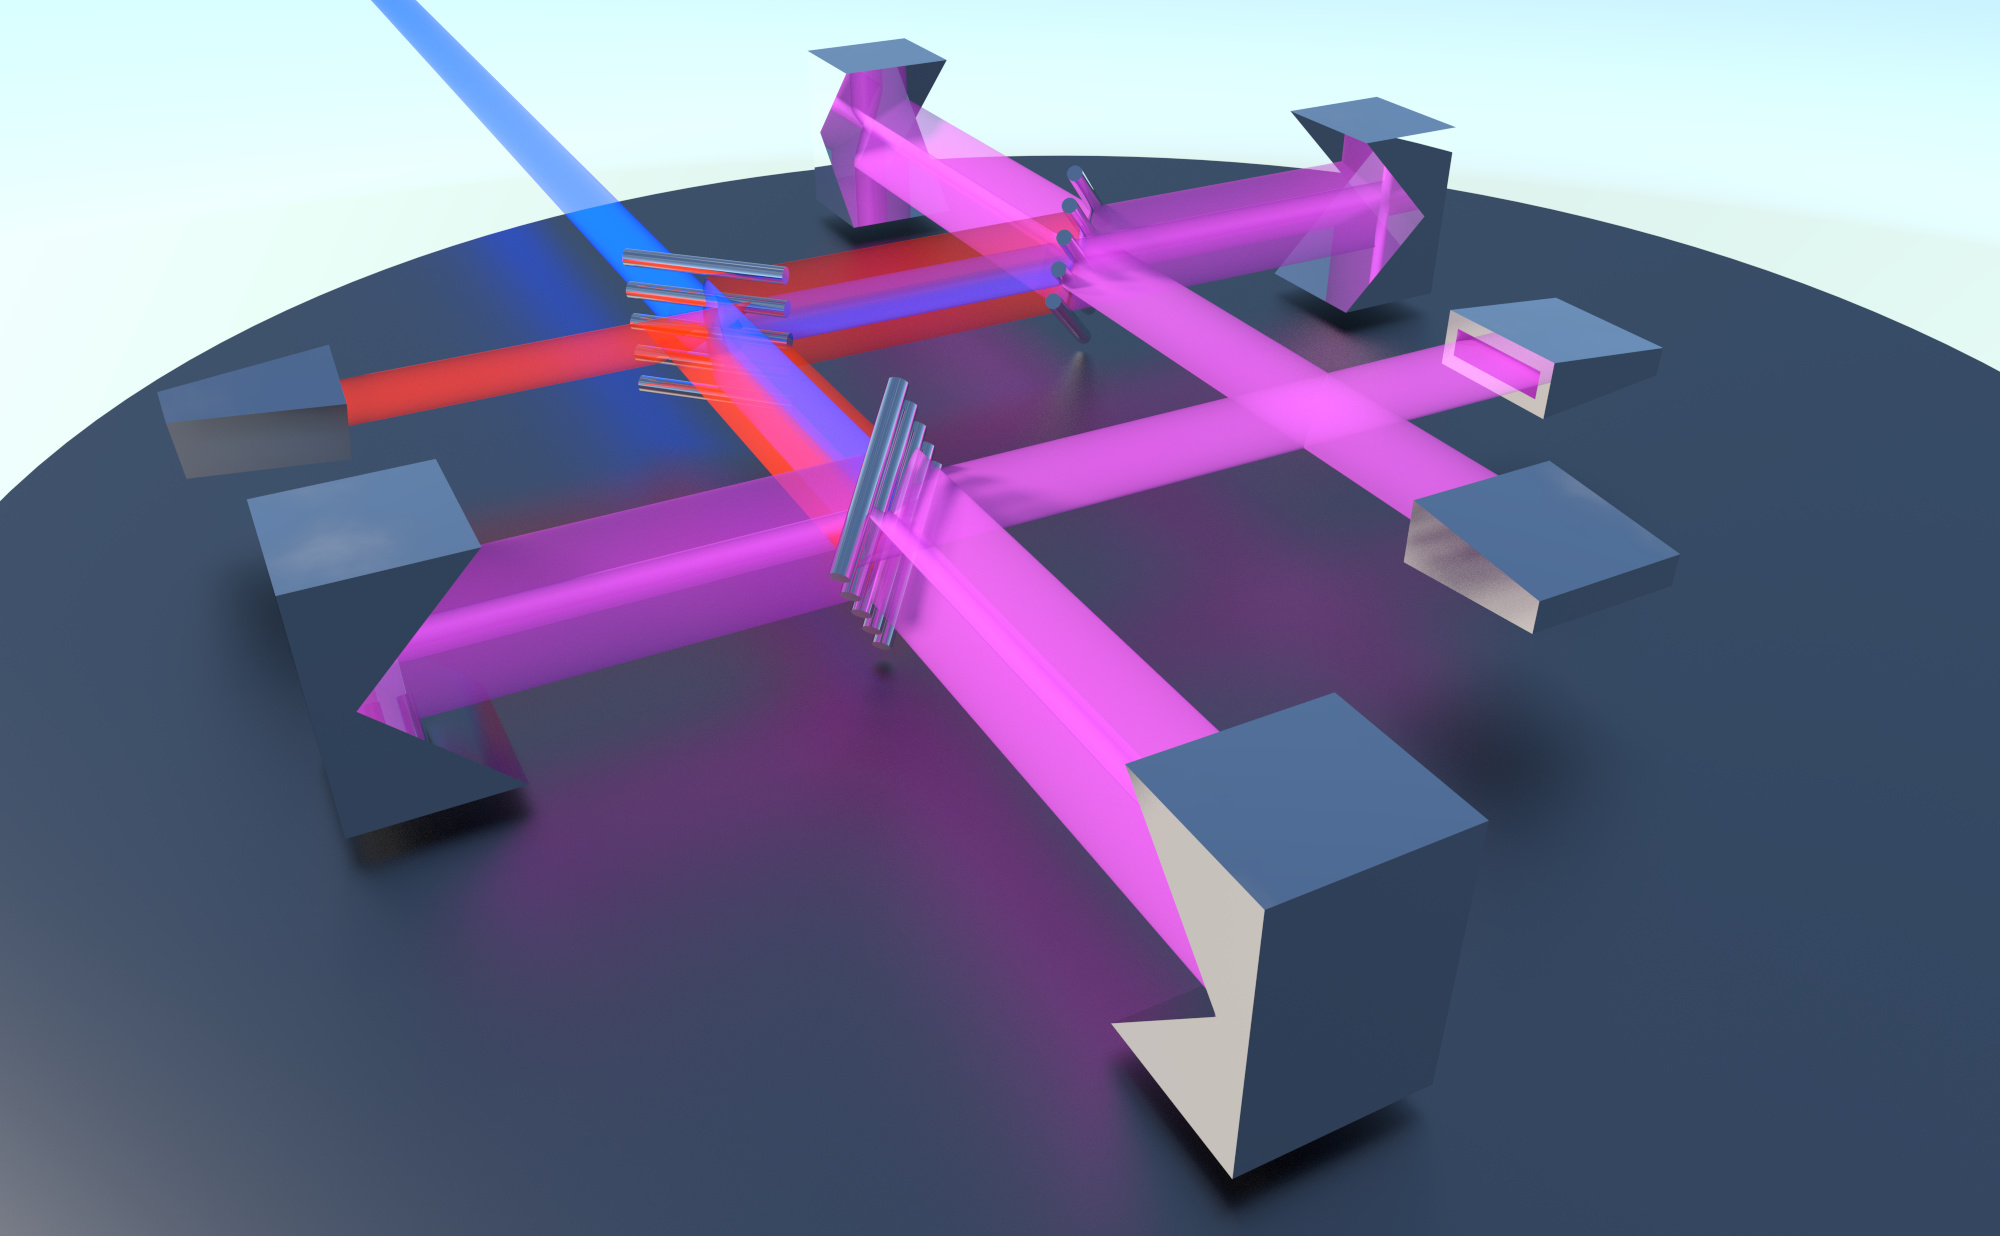
\includegraphics[width=\textwidth]{diplexer_render_lowres}
    \caption{
        Schematic 3D representation of the diplexer units in HIFI.
        The blue beam represents the signal from the sky, the red beam is the LO signal,
        and the purple beams are a superposition of the two.
        \emph{First}, the LO and sky signal are split in two by a wire-grid polarizer.
        The polarization of the beams is represented by their tilt.
        \emph{Second}, the LO and sky beams have their polarizations lined-up by the diplexers.
        Each diplexer is made of one wire-grid polarizer and two rooftop mirrors.
        \emph{Finally}, the combined beams of the LO and the sky enter the horns to be mixed.
    }
    \label{fig:diplexer_render}
\end{figure}



%=============================================================================
\subsection{IF chain and backends}

The IF signal produced by the mixers is fed into two spectrometers:
the digital autocorrelation High Resolution Spectrometer (HRS) and
the acousto-optical Wide Band Spectrometer (WBS).

There are two identical WBS and two identical HRS: one per polarization.

The WBS resolution is fixed at \SI{1.1}{\mega\hertz} with a channel every \SI{0.5}{\mega\hertz}.
Its instantaneous bandwidth covers the whole IF range of 4 to \SI{8}{\giga\hertz}.

The HRS offers up to four bands that can be placed anywhere inside the IF range.
The width of these bands and the spectral resolution is variable: the higher the resolution, the narrower the bandwidth (see~\cref{tab:wbs_hrs}).

\begin{table}[hb]
    \centering
    \begin{tabular}{lrrr}
    \toprule
    Spectrometer and mode & 
    CS [\si{\kilo\hertz}]
    &
    SR [\si{\kilo\hertz}]
    &
    BW [\si{\mega\hertz}]\\
    \midrule
    HRS High resolution   &  67 &  135 & $1 \times \phantom{0}250$\\
    HRS Medium resolution & 134 &  270 & $2 \times \phantom{0}250$\\
    HRS Low resolution    & 270 &  539 & $4 \times \phantom{0}250$\\
    HRS Wide band         & 540 & 1078 & $4 \times \phantom{0}500$\\
    \midrule
    WBS                   & 500 & 1100 & $1 \times 4000$\\
    \bottomrule
    \end{tabular}
    \caption{
        Summary of the spectral properties of the HIFI HRS and WBS.
        CS is the channel spacing,
        SR is the spectral resolution (Hanning apodization) and
        BW is the bandwidth.
        Credit: \textcite{belgacem2004high}.
    }
    \label{tab:wbs_hrs}
\end{table}


%#############################################################################
\FloatBarrier
\section{Coherence, cavities, standing waves and interferences}
\sectionmark{Coherence, cavities and interferences}
\label{sec:coherence}

%=============================================================================
\subsection{Vocabulary}

Ripples and Standing waves are side-effects of coherence and cavities.

When light enters a cavity, some of the light is reflected, some of the light is transmitted, some of the light is lost (heat) and some of the light is stored inside the cavity.

The light stored inside the cavity can be seen in two ways:
either as a superposition of an infinity of waves traveling in both directions,
or as a single wave that is not traveling.
Both interpretations are equally valid, both are solutions to Maxwell's equations.
It is a matter of perspective.
When we consider the light trapped in the cavity as a single wave, its nodes and crests do not move: the oscillation stands there, fixed in space.
This is what we call a ``standing wave''.

Astronomers and engineers alike tend to abuse the language slightly for the sake of brevity and because the context is often clear.
Some would say that the spectra shown in~\cref{fig:ripples} have a standing wave, using the word ``standing wave'' to mean ``ripple''.
Some would say that standing waves are responsible for the ripple, using ``standing wave'' instead of ``interferences''.

In truth, both ripples and standing waves are results of interferences.
The ripple is a frequency-dependent modulation of the light exiting the cavity, and the standing wave corresponds to the light that remains in the cavity for a given frequency.
The three concepts ``ripple'', ``standing wave'' and ``interference in a cavity'' are tightly coupled and go together, one cannot have one without the others.
This is why this slight abuse of language is often acceptable.
However, for the sake of clarity, I choose my words carefully.


%=============================================================================

\subsection{Coherence}

The notion of coherence refers to the degree of correlation, described in a specific mathematical fashion, between two signals observed at different points in time and/or space.
When the amplitude, the phase and the polarization of a wave changes only slowly with time, the amplitude, phase and polarization of that wave at any one time is strongly correlated with those of that same wave at considerably earlier or later times.
Between these two moments, the wave may have undergone several reflections on the various optical elements that make the instrument.
These reflections can make the wave overlap itself in space, and the strong degree of phase correlation implies that the wave interferes with itself.

The ``coherence time'' measures the time scale over which a wave remains strongly correlated.
The coherence time~$\tau$ of a signal is related to its bandwidth~$\Delta f$ by
\begin{equation}
    \tau = \frac{1}{\Delta f} \text{.}
\end{equation}
The coherence length equals $c\tau$, where $c$ is the speed of the wave in the medium.
\Cref{fig:coherence} illustrates the relation between bandwidth and coherence time/length.

\begin{figure}
    \centering
    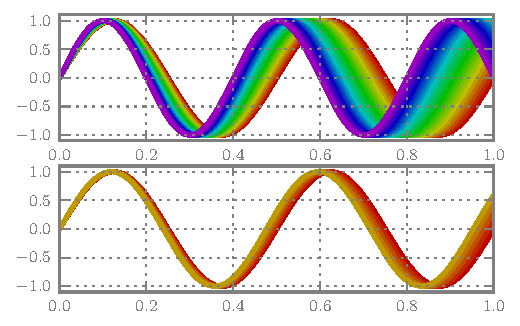
\includegraphics[width=.8\textwidth]{coherence}
    \caption{
        Coherence time is a function of bandwidth.
        Signals with a narrow bandwidth remain in phase longer.
        Colors represent frequencies.
        The $x$ axis can represent either time or space and the $y$ axis represents the amplitude of the electric field for the corresponding frequency, both in arbitrary units.
        After propagating to $x=0.9$, the red and purple frequencies of the top-plot signal have opposite phase; a detector that cannot discriminate between them adds up their contribution to 0.
        In the bottom plot, the signal is still very much in phase at $x=0.9$
        because it has a narrower bandwidth.
    }
    \label{fig:coherence}
\end{figure}

\begin{figure}
    \centering
    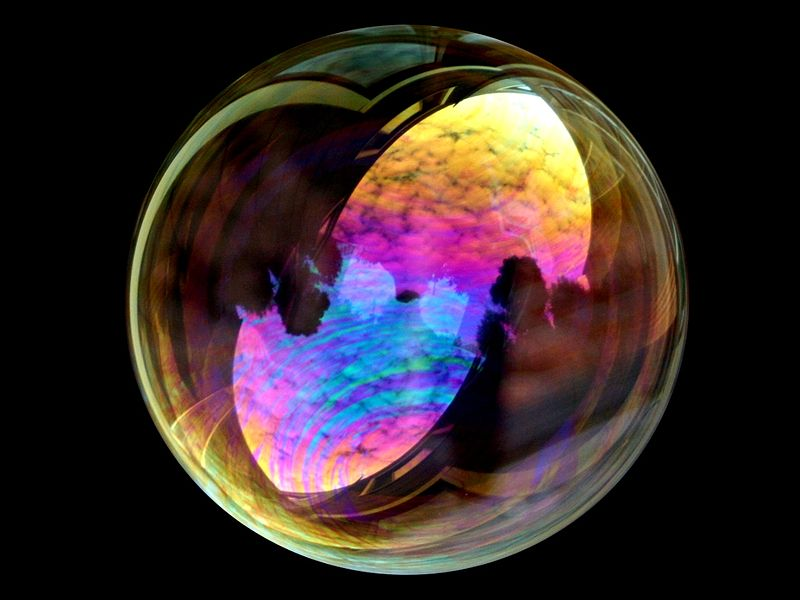
\includegraphics[width=.8\textwidth]{soap_bubble_sky}
    \caption{The iridescence of soap bubbles results from interferences inside the thin film of soap.
    Credit: Brocken Inaglory, 2007, License: (CC~BY-SA~3.0).
}
    \label{fig:soap_bubble}
\end{figure}

%=============================================================================

\subsection{Cavities}

Any two surfaces that face each other via at least one optical path form a cavity.
Light reflect back and forth between the two surfaces.
For a cavity to give rise to interferences, the cavity must be short when compared to the coherence length\index{coherence length} of a wave.
In that case the wave remains coherent during its round trips inside the cavity.
This allows the wave to interfere with itself.
There is no interference without coherence.

Cavities exist in the optical path of HIFI.
The optical components are not perfect: calibration black bodies are gray, wire-grid polarizers leak, mirrors are not perfect conductors, LO and mixer horns have coupling efficiencies lower than 1, the mixers are slightly reflective, the rooftop mirror planes do not intersect at right angle, etc.
For example, the mixer and the local oscillator form a cavity.
So do the mixer and the cold calibration load, or the mixer and the roof-top mirrors of the diplexer units.
Any pair of surface that somehow face each other, even via other surfaces, form a cavity.

There are also cavities in the IF chain side of HIFI, between the mixers and the backends.
Bands~6 and 7 of HIFI lack isolators between the mixer and the IF-amplifiers.
This allows the mixer to see the amplifier and creates a cavity.
The case of the interferences on the IF-side of the mixer in Bands~6 and~7 has been investigated by~\textcite{higgins2011}.
I focused my work on the interferences in the optics.

Each WBS channel has a bandwidth $\Delta f = \SI{1.1}{\mega\hertz}$,
which yields $\tau = 1 / \Delta f = \SI{909}{\nano\second}$.
By multiplying by the speed of light, we find that the WBS has a coherence length of~\SI{273}{\meter}.
This means that, as long as a signals travels significantly less than~\SI{273}{\meter}, it is coherent as far as the WBS is concerned.
The path lengths inside HIFI are much shorter than~\SI{273}{\meter};
for example, the distance between the LO and the mixers is about~\SI{1}{\meter}.
When the bandwidth is so narrow, the thermal noise of the astronomical source, the calibration loads and the local oscillator is coherent%
\footnote{If fully polarized, which is rarely the case for noise.  This is not a problem: \cref{sec:chapter2} describes how an unpolarized wave can be modeled as a superposition of polarized waves.}
 and qualify as ``narrow band Gaussian noise signals''~\parencite{siegman1986lasers}.
The high spectral resolution of HIFI makes it a coherent instrument, therefore sensitive to interferences.

In comparison, the spectrometer of PACS operates typically at \SI{3}{\tera\hertz} with a resolution of 2000: $\Delta f = \SI{1.5}{\giga\hertz}$ which gives a coherence length of~\SI{20}{\centi\meter}, therefore a cavity length at most equal to~\SI{10}{\centi\meter}.
PACS is considerably less coherent than HIFI but can still suffer from interferences in small cavities.

%=============================================================================
\subsection{Frequency-dependence}

The length of a cavity (and the properties of all the material involved), determines which wavelengths interfere constructively and which ones interfere destructively.
This dependence on the wavelength explains the periodicity ripples.
As a first order simplification, the period $F$ of a ripple and the length $d$ of a cavity are linked by
\begin{equation}
    F = \frac{c}{2d}
\end{equation}
where $c$ is the speed of light in the cavity.

\Cref{fig:soap_bubble} illustrates the wavelength-dependence of the effect of a cavity in a familiar case: that of the iridescence of a soap bubble.
The thickness of the thin layer of soap at any given point, combined with the direction of propagation of the light at that point, determines which wavelengths interfere positively or destructively in the direction of your eye.
The spectrum reflected and transmitted by the bubble is profoundly modified by the soap cavity.





%=============================================================================
\subsection{Intensity calibration}
\label{sec:intensity_calibration}

%-----------------------------------------------------------------------------
\subsubsection{Chopper wheel method}
The intensity calibration of HIFI follows the general principle of the chopper wheel method described by~\textcite{ulich1976absolute,kutner1981recommendations}.
In a few words, a detector converts the power $J$ received from a source into an arbitrary quantity $c=aJ+b$ where $b$ is the background emission and $a$ the bandpass.
In order to retrieve $J$ from $c$, we need to determine the value of the two unknowns $a$ and $b$.
We determine $b$ by coupling the detector to an empty region of the sky and $a$ by coupling it to calibration sources of known power (hot/cold black bodies).

Taking four spectra (source $s$, reference $r$, hot $h$ and cold $c$) yields four equations.
\begin{equation}
    \begin{aligned}
        c_s &= a_s J_s + b_s\\
        c_r &= a_r J_r + b_r\\
        c_h &= a_h J_h + b_h\\
        c_c &= a_c J_c + b_c
    \end{aligned}
\end{equation}
We make assumptions.
The emission $J_r$ of the reference position is known (0, or any known continuum intensity).
The emissions $J_h$ and $J_c$ of the black bodies are known (Planck's law applied to known temperatures $T_h$ and $T_c$).
The optical gain is the same for all: $a_s = a_r = a_h = a_c = a$.
The background is the same for the source and the reference (same main dish and same atmosphere): $b_s = b_r = b_1$.
Likewise, $b_h = b_c = b_2$ (no main dish, less atmosphere).
\begin{equation}
    \left.
    \begin{aligned}
        c_s &= a   J_s + b_1\\
        c_r &= a   J_r + b_1\\
        c_h &= a   J_h + b_2\\
        c_c &= a   J_c + b_2
    \end{aligned}
    \right\rbrace
    J_s = J_r +
    \underbrace{
        \frac{J_h - J_c}{c_h - c_c}
    }_{a}
    (c_s - c_r)
    \label{eq:ideal_calibration}
\end{equation}

There is a problem: these equations assume that the instrument is single-sideband and incoherent.
HIFI is a coherent double-sideband receiver, some of the assumptions made in the previous paragraph do not hold.

%-----------------------------------------------------------------------------
\subsubsection{Impact of interferences on HIFI's calibration}

Because HIFI is coherent, interferences modulate the bandpass $a$ and the background $b$ differently for each optical configuration.
If the telescope slews between the source and reference positions on the sky then nothing inside the telescope changes and the assumption $a_s=a_r$ and $b_s=b_r$ still holds.
Despite a maximal slewing speed of \SI{7}{\arcmin\per\second}, it actually takes Herschel~\SI{20}{\second} to slew by~\SI{3}{\arcmin} because of a slow acceleration and a stabilization time.
The Allan times (a measure of mixer stability) of HIFI can be low: between 0 and \SI{300}{\second} depending on the mixer band and the intent of the astronomer~\parencite{ossenkopf2008stability}.
Ideally, a source--reference observation cycle should take at most one third of the Allan time.
Obviously, slewing is not always an option.
Even when slewing is an option, it is in some cases a waste of time.

An alternative to slewing the whole satellite is to tilt the chopper, which takes only a fraction of a second.
Tilting the chopper changes the optics, therefore $a_s \ne a_r$ and $b_s \ne b_r$.

It is possible to combine chopping and slewing so that both the source and the reference are observed in both chopper positions.
This adds two equations to the system with which we can properly cancel $a$ and $b$ for the sky.
HIFI provides this observing mode, named ``dual beam switch''.
With HIFI, the reference position is not necessarily a point on the sky, it can be the cold load itself (``load chop'').
Alternatively, the ``frequency switch'' observing mode alternates between two LO frequencies, bringing continuum where there was a line and vice-versa.
\Textcite{ossenkopf2002intensity} details the various observing modes of HIFI and their calibration.

Even with a dual beam switch observing mode, the background and the bandpass differ in the hot, cold and sky spectra.
As a result, \cref{eq:ideal_calibration} does not cancel them properly and the value of $J_s$ is incorrect: ripples may appear on the baseline, the line intensities and/or profiles may be affected.

The problem is made worse because HIFI is also double-sideband instrument: the number of parameters doubles.
With the indices $l$ and $u$ denoting lower-sideband and upper-sideband values, the chopper wheel calibration scheme produces a system of equations that is greatly underdetermined.

\begin{equation}
    \begin{array}{*{11}{@{\,}l@{}}}
        c_s &=& a_{sl} &J_{sl} &+& b_{sl} &+& a_{su} &J_{su} &+& b_{su} \\
        c_r &=& a_{rl} &J_{rl} &+& b_{rl} &+& a_{ru} &J_{ru} &+& b_{ru} \\
        c_h &=& a_{hl} &J_{hl} &+& b_{hl} &+& a_{hu} &J_{hu} &+& b_{hu} \\
        c_c &=& a_{cl} &J_{cl} &+& b_{cl} &+& a_{cu} &J_{cu} &+& b_{cu}
    \end{array}
\end{equation}

One solution to the proliferation of parameters would be to use natural sources on the sky, of well~known flux, as calibration sources.
This is impractical: these sources are few, they may require long slewing times, and they may even be out of reach of Herschel (Herschel must keep its solar panel toward the sun at all time).

In order to retrieve the astronomical signal $J_{sl}$ and  $J_{su}$
from the four spectra $c_s$, $c_r$, $c_h$ and $c_l$, one needs to know the gain of the mixer and the optics in every situation.
Without that knowledge, one is forced to make assumptions.
Typically, the HIFI calibration pipeline assumes that the gain of the system is the same in both sidebands: it ignores interferences in the optics and IF-dependence of the mixer gain.

%\begin{samepage}
We define the ``sideband gain ratio'' $\text{SBR}$ of the system with
\begin{equation}
    \text{SBR} = \frac{a_u}{a_l + a_u} \label{eq:sbr}
\end{equation}
where $a_l$ and $a_u$ are the LSB and USB system gains.
The ideal value of the sideband gain ratio is~\num{0.5}, indicating a balanced receiver.
Deviations from~\num{0.5} indicate a ``sideband imbalance''.
A channel of a HIFI spectrum is USB-dominated if the sideband ratio of this channel is greater than~\num{0.5}, LSB-dominated otherwise.
%\end{samepage}
\Cref{fig:lo_scan_of_ripple} presents a simple simulation of the sideband ratio over the IF for a few LO frequencies.
It illustrates that the amplitude and the phase of the LSB and USB ripples become degenerated when folded \footnote{This results from the sum--to--product trigonometric identity~$\cos(a)+\cos(b) \equiv 2 \cos(\nicefrac{a+b}{2}) \cos(\nicefrac{a-b}{2})$.}.
Strong ripples can interfere destructively with themselves and weak ripples can interfere constructively.

\begin{figure}[bp]
    \centering
    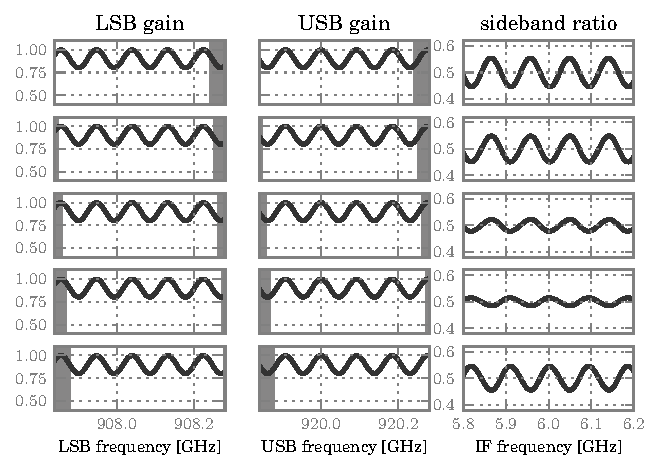
\includegraphics{lo_scan_of_ripple}
    \caption{
        Simple simulation of the LO-frequency dependence of the sideband gain ratio.
        \emph{Rows}:
            Each row corresponds to one~LO frequency.
        \emph{Left and center columns}:
            The LSB and USB optical gains are modulated by a ripple.
            The background color indicates whether a frequency
            contributes to the IF (white) or not (gray).
            The ripple does not depend on the LO~frequency but the window does.
        \emph{Right column}:
            The sideband gain ratio,
            defined by
            $\text{SBR}=\frac{\text{USB gain}}{\text{LSB gain}+\text{USB gain}}$,
            depends on the LO~frequency:
            the LSB and USB ripples interfere.
    }
    \label{fig:lo_scan_of_ripple}
\end{figure}

There are two main contributions to these gains $a_l$ and $a_u$:
the mixer gain itself ($a_{ml}$ and $a_{mu}$)
and the optics ($a_{ol}$ and $a_{ou}$), related by
$a_l = a_{ml} a_{ol}$ and $a_u = a_{mu} a_{ou}$.

In HIFI, the LSB and USB are separated by \num{8} to~\SI{16}{\giga\hertz}
which is a significant fraction (\SI{7}{\percent}) of the total bandwidth of the mixers (\SI{160}{\giga\hertz}),
therefore an IF-dependence of the mixer sensitivities is expected.
However, it is reasonable to expect that the mixer gains do not vary when the optics change: they are independent from the chopper position and are the same for the integrations on the source, reference and calibration loads (provided these integrations take place within the Allan time).

The gain of the optics can depend on the IF for several reasons:
different beam sizes at different frequencies (negligible), dispersive%
\footnote{
    Dispersion is the phenomenon in which the phase velocity of a wave depends on its frequency; a dispersive element in a cavity makes the optical length of a cavity a function of frequency.
}
components (wire grid polarizers for instance), or destructive interferences.

\Cref{fig:sbr_effect} illustrates the effect that sideband ratio imbalances can have on the intensity calibration of HIFI.
The same line, observed eight times with eight LO frequencies, should result in eight spectra that overlap within the noise.
This is not the case.
The sideband gain changes with the LO setting.
There are two possible reasons for these changes:
\begin{enumerate}[noitemsep,nolistsep]
    \item With each LO setting, the line is placed at a different intermediate frequency.  Since the sideband ratio is IF-dependent, the output of the mixer varies.
    \item The LO power changes for each LO frequency in order to optimally pump the mixer.
    This changes some properties of the mixer.
\end{enumerate}
Both effects can happen simultaneously.

\begin{figure}
    \centering
    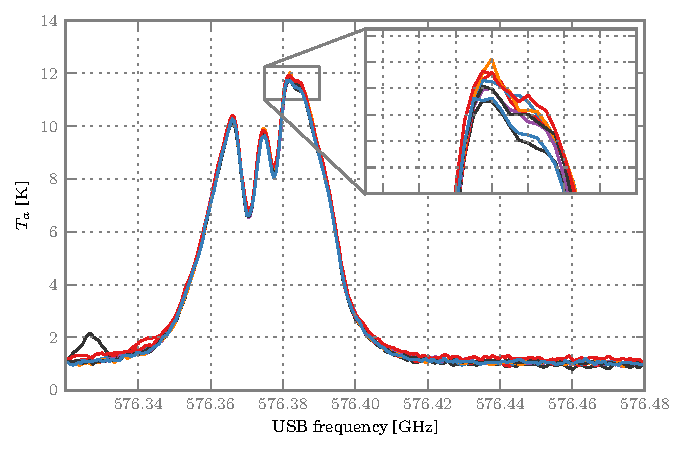
\includegraphics{sbr_effect}
    \caption{
        Impact of the sideband ratio uncertainty.
        The same line is observed with 8 LO frequencies separated by~$\approx \SI{50}{\mega\hertz}$.
        Variations of the sideband ratio are responsible for the spread of peak intensity.
        The black peak that stands out at the bottom left of the spectrum is a minor spectral line from the LSB, which entered this region of the IF at a given LO setting.
        HSA obsid 0x5000326d.
    }
    \label{fig:sbr_effect}
\end{figure}

\Cref{fig:sbr_effect} suggests that observing a line of known intensity should constrain the sideband ratio.
This has been done during the Instrument-Level Tests in 2006 using a gas cell designed by \textcite{teyssier2004multi}, through which HIFI measured absorption lines of \ce{^{12}CO}, \ce{^{13}CO}, \ce{CH3CN}, \ce{H2O} and \ce{OCS}.
This data, combined later with flight data, was analyzed over years.
\Cref{fig:sideband_ratio} presents a summary of these SBR measurements~\parencite{higgins2010calibration,higgins2014effect}.
With one point per LO frequency, these results do not consider the IF-dependency of the SBR.
Furthermore, the gas cell data was acquired before HIFI received new attenuators in its LO path~\parencite{jellema2008flight}; these attenuators have considerably reduced interferences inside the LO--mixer cavities and improved the stability of the mixers, which probably had a beneficial impact on the SBR by reducing its IF variability.
Exploiting these results is therefore difficult.

Despite considerable efforts, the sideband ratio of HIFI remains one of the major sources of uncertainty in the intensity calibration~(see~\cref{sec:intensity_calibration}).

The work that I present in this thesis is an attempt at approaching this problem from a different angle.
By modeling the physics of interferences in the optics, one should be able to determine the values of the LSB and USB gains of the optics, not only for each LO setting, but for each IF channel.

\begin{figure}[hbp]
    \centering
    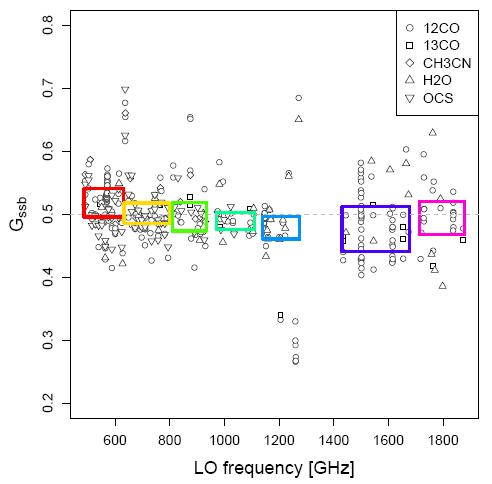
\includegraphics[width=.75\textwidth]{sideband_ratio}
    \caption{
        Sideband ratio as a function of LO frequency.
        Each box corresponds to a LO band, their vertical extension delineate all data falling within the first and third quartile.
        Credit: \textcite{higgins2014effect}.
    }
    \label{fig:sideband_ratio}
\end{figure}

\begin{table}[p]
    \centering
    \begin{tabular}{lcccc}
        \toprule
        Error source           & Band 1/2 & Band 3/4 & Band 5 & Band 6/7 \\
        \midrule
        Sideband ratio         & 3--4     & 4--6     & 4--6   & 5--8     \\
        Hot load coupling      & <1       & <1       & <1     & <1       \\
        Cold load coupling     & <1       & <1       & <1     & <1       \\
        Hot load temperature   & <1       & <1       & <1     & <1       \\
        Cold load temperature  & <1       & <1       & <1     & <1       \\
        Planetary model error  & <3       & <3       & <3     & <3       \\
        Beam Efficiency        & <5       & <5       & <10    & <5       \\
        Pointing               & <1       & <2       & <2     & <4       \\
        Optical interferences  &  4       & 4        & 3      & 3        \\
        \bottomrule
    \end{tabular}
    \caption{
        Overall error budget of HIFI~\parencite{hifiobserversmanual}.
        Percentage intensity uncertainty associated with each component of the error budget.
    }
    \label{tab:calibration_errors}
\end{table}

\begin{table}[p]
    \centering
    \begin{tabular}{l *{7}{C{0.8cm}} }
        \toprule
            Band & 1 & 2 & 3 & 4 & 5 & 6 & 7 \\
        \midrule
            loads -- mixer    & $ 4$ & $ 3$ &    $2$ &    $1$ & $1$ & $<1$ & $<1$ \\
            LO -- mixer       & $<1$ & $<1$ & $2$--$4$ & $2$--$4$ & $3$ &  $3$ &  $3$ \\
            rooftops -- mixer & -    &  -   & $1$--$2$ & $1$--$2$ & - & $<1$ & $<1$ \\
        \midrule
            overall           & $4$ & $3$ & $4$ & $4$ & $3$ & $3$ & $3$\\
        \bottomrule
    \end{tabular}
    \caption{
        HIFI Intensity calibration uncertainty due to interferences~\parencite{risacher2011standingwaves}.
        Values are given in percent.
        Bands 1, 2 and 5 have no rooftop mirror, therefore no associated ripple.
    }
    \label{tab:ripple_errors}
\end{table}

\begin{table}[p]
    \centering
    \begin{tabular}{lcc}
        \toprule
            path & cavity length [\si{\milli\meter}] & ripple period [\si{\mega\hertz}]\\
        \midrule
            cold load -- mixer & $\approx\num{1530}$ &  98\\
            hot load -- mixer  & $\approx\num{1625}$ &  92\\
            LO -- mixer        & $\approx\num{1490}$ & 100\\
            rooftops -- mixer  & $\approx\num{ 240}$ & 620\\
            secondary -- mixer & $\approx\num{4160}$ &  35\\
        \bottomrule
    \end{tabular}
    \caption{
        Summary of the main HIFI ripples~\parencite{risacher2011standingwaves}.
    }
    \label{tab:ripple_periods}
\end{table}



%-----------------------------------------------------------------------------
\FloatBarrier
\subsubsection{Error budget}
The absolute calibration accuracy of HIFI is at least~\SI{10}{\percent}, with a goal of~\SI{3}{\percent}.
\Cref{tab:calibration_errors} summarizes the origin of the actual calibration uncertainties for the seven bands.
Sideband ratio and optical interferences stand out in this table for being amongst the biggest contributors to the uncertainty.
In HIFI, the problem of the sideband ratio and that of interferences are actually related:
interferences in the optics modulate the optical gain differently in LSB and USB, therefore interferences contribute to the sideband ratio imbalance.
\Cref{tab:ripple_errors,tab:ripple_periods} list the periods of ripples commonly measured on HIFI spectra, their matching cavity lengths, and their impact on the error budget.






%#############################################################################
\section{Modeling Interferences}

Because the far-infrared is between the microwave and optical domains of the electromagnetic spectrum, many modeling techniques developed for microwave or optical engineering can be applied to the far-infrared.

From the optical side, we can use ray tracing~\parencite{spencer1962general}.
Ray tracing often assumes that the light is incoherent and propagates along infinitely-thin beams.
Laser theory introduces some tools to deal with coherence and the self-diffraction of the beam~\parencite{siegman1986lasers}.
These theories make use of matrices to describe changes to the degree of polarization of light (Stokes parameters, Müller matrices, Jones matrices), and to the geometry of the beam (ray optics or Gaussian beams ABCD matrices)~\parencite{goldsmith1998quasioptical}.

From microwave circuits and waveguides theory, we can use the many types of 2--by--2 matrices that link voltage and current for two-ports networks:
the two categories \{voltage, current, relations between them\} and \{electric field, magnetizing field, relations between them\} are isomorphic.
There are also scattering matrices which allow for more than two ports~\parencite{pozar2009microwave}.

\Cref{tab:tools} presents a brief overview of different tools used to model optical or microwave systems.
Suffice to say that, short of solving Maxwell's equations in four dimensions, there is no magic bullet that treats all aspects of the problem at once.
Some tools are designed explicitly to model polarization, others can be tweaked in order to include it, and other tools are just not made for that.

The modeling technique that I developed has its own limitations but is a sound first-order approximation.
It combines several techniques inspired from circuit theory (notably scattering and Jones matrices), extends them to work in three dimensions, and includes an algorithm to solve the steady state of optical systems of any size and complexity.
For now, it ignores the geometry of the beam: I assume that the waves are plane and the signals are mono-mode, and focus on the intensity, phase and polarization coherence of these waves.
This approximation guarantees that the system can be described with linear equations, and guarantees that it has a closed-form solution for the steady state.

%\Textcite{whyborn2002standingwaves} mentions that interferences can not only modulate the optical coupling between a source and a detector, but also the intrinsic noise of the mixer itself.

\begin{sidewaystable}[hbtp]
    \centering
    {\footnotesize
    \rowcolors{1}{gray!20}{}
    \begin{tabularx}{\textwidth}{X|X X X X X X}
        \toprule
                                          & Ray tracing & Ray optics ABCD matrix & 2-port network matrices & Scattering matrix & Jones matrix & Müller matrix  \\
        \midrule
        Intensity/power                   & yes         & no                     & yes                     & yes               & yes          & yes            \\
        Phase (coherence)                 & yes         & yes                    & yes                     & yes               & yes          & no             \\
        Polarized                         & yes         & possible               & irrelevant              & possible          & yes          & yes            \\
        Unpolarized                       & yes         & yes                    & irrelevant              & possible          & no           & yes            \\
        Direction of propagation          & yes         & a bit                  & no                      & no                & no           & no             \\
        Gaussian beam width and curvature & no          & yes                    & no                      & no                & no           & no             \\
        Gaussian beam modes               & no          & yes                    & no                      & no                & no           & no             \\
        More than 2 ports                 & yes         & no                     & no                      & yes               & no           & no             \\
        Cascade-able                      & yes         & yes                    & some                    & no                & yes          & yes            \\
        Steady-state                      & no          & no                     & yes                     & yes               & no           & no             \\
        \bottomrule
        \end{tabularx}
    }
    \rowcolors{1}{}{}
    \caption{\label{tab:tools}No tool or framework satisfies all the criteria.}
\end{sidewaystable}


%#############################################################################
\section{Layout of the thesis}

\Cref{sec:chapter2} begins by diving into the physics and mathematics of coherence, cavities and interferences.
After an introduction to cavities, I present a new technique to predict the gain of a coherent system of arbitrary complexity.
First, I describe the mathematics of this technique:
assuming that optical elements can be represented with matrices, I show how to predict the phase and amplitude of the electric field at any point inside the system.
This method solves directly for the steady state and takes into account the infinite reflections between every pair of elements along every possible path.
Second, I provide a complete implementation of these technique with pseudo-code.
These algorithms can be painlessly translated, often word for word, into common high-level programming or data analysis language.
Third, I present a library of specific optical elements: parametrized matrices describing HIFI components such as rooftop mirrors and wire grid polarizers.

In \cref{sec:chapter4} I create a model of HIFI Band~1 that I compare to actual HIFI data.
The goal is to predict qualitatively or quantitatively the optical gain of HIFI, ideally removing unknowns from the calibration equation.
Constraining the model parameters proves to be a difficult task, especially when this is done after the end of the mission.
Future instruments should have more success by performing some dedicated tests and observations.

In \cref{sec:chapter5}, using a series of HIFI observations designed specifically for this purpose, I study the impact of interferences and thermal noise uncertainties on a real astronomical case: the determination of the kinetic temperature and density of~\ce{H2} deep into the core of the massive young stellar object S140~IRS1.


%#############################################################################
\FloatBarrier
%\clearpage
%\printbibliography[heading=subbibliography]
%\end{refsection}
